\pdfinfoomitdate=1
\pdftrailerid{}
\pdfsuppressptexinfo=15
\documentclass[11pt]{article}
\usepackage[T1]{fontenc}
\usepackage{lmodern}
\usepackage[margin=1in]{geometry}
\usepackage{amsmath,amssymb,amsthm,mathtools}
\usepackage{microtype}
\usepackage{enumitem,booktabs,array,graphicx}
\usepackage{flafter}
\usepackage[dvipsnames]{xcolor}
\usepackage{tikz}
\usetikzlibrary{arrows.meta,positioning,fit,calc,matrix,patterns,decorations.pathreplacing,shapes.geometric}
\usepackage[numbers,sort&compress]{natbib}
\usepackage{hyperref}
\hypersetup{colorlinks=true,linkcolor=MidnightBlue,citecolor=MidnightBlue,urlcolor=MidnightBlue,
  pdftitle={A translational tile with no fully periodic tiling in dimension three},pdfauthor={OpenAI}}
\usepackage[capitalise,nameinlink,noabbrev]{cleveref}
\newtheorem{theorem}{Theorem}[section]
\newtheorem{lemma}[theorem]{Lemma}
\newtheorem{proposition}[theorem]{Proposition}
\newtheorem{corollary}[theorem]{Corollary}
\theoremstyle{definition}
\newtheorem{definition}[theorem]{Definition}
\theoremstyle{remark}
\newtheorem{remark}[theorem]{Remark}
\newtheorem{example}[theorem]{Example}
\usepackage{needspace,etoolbox}
\makeatletter
\newcommand{\statementspace}{%
  \if@nobreak\else\par\Needspace{4\baselineskip}\fi}
\makeatother
\BeforeBeginEnvironment{theorem}{\statementspace}
\BeforeBeginEnvironment{lemma}{\statementspace}
\BeforeBeginEnvironment{proposition}{\statementspace}
\BeforeBeginEnvironment{corollary}{\statementspace}
\BeforeBeginEnvironment{definition}{\statementspace}
\BeforeBeginEnvironment{remark}{\statementspace}
\BeforeBeginEnvironment{example}{\statementspace}
\numberwithin{equation}{section}
\crefname{theorem}{Theorem}{Theorems}
\crefname{lemma}{Lemma}{Lemmas}
\crefname{proposition}{Proposition}{Propositions}
\crefname{corollary}{Corollary}{Corollaries}
\crefname{definition}{Definition}{Definitions}
\crefname{remark}{Remark}{Remarks}
\crefname{section}{Section}{Sections}
\crefname{figure}{Figure}{Figures}
\crefname{equation}{Equation}{Equations}
\newcommand{\Z}{\mathbb Z}
\newcommand{\R}{\mathbb R}
\newcommand{\F}{\mathbb F}
\newcommand{\N}{\mathbb N}
\newcommand{\Zmod}[1]{\Z/#1\Z}
\newcommand{\Fp}{\mathbb F_p}
\DeclarePairedDelimiter{\abs}{\lvert}{\rvert}
\DeclarePairedDelimiter{\norm}{\lVert}{\rVert}
\setlist{topsep=4pt,itemsep=3pt,parsep=0pt}
\setlength{\emergencystretch}{1.5em}
\title{A translational tile with no fully periodic tiling\\in dimension three}
\author{OpenAI}
\date{September 23, 2026}

\begin{document}
\maketitle
\begin{abstract}
We construct a finite translational tile in $\Z^3$ that admits tilings but no fully periodic tiling. Its unit-cube thickening has the same property in $\R^3$, even when arbitrary real translations are allowed. This gives a negative resolution of the periodic tiling conjecture in dimension three.
\end{abstract}

\section{Introduction}\label{sec:introduction}
For subsets $A,F$ of an abelian group $G$, write $A\oplus F=G$ when every element of $G$ has a unique expression $a+f$ with $a\in A$ and $f\in F$. A finite nonempty set $F$ is a \emph{translational tile} if such a set $A$ exists. A tiling is \emph{fully periodic} if $A$ is invariant under a subgroup of finite index in $G$. In $\R^3$, a bounded measurable set of positive measure tiles by translations when its translates partition space up to null sets; full periodicity means that its translation set is invariant under a lattice of full rank. Throughout this paper, ``periodic'' means fully periodic.

The periodic tiling conjecture asks whether every translational tile
admits a periodic tiling. An explicit Euclidean formulation appears in
\citet[p.~346]{LagariasWang}. Our conclusion in dimension three is the
following.

\begin{theorem}\label{thm:main}
There is a finite nonempty set $T\subset\Z^3$ such that:
\begin{enumerate}[label=\textup{(\roman*)}]
\item $T$ tiles $\Z^3$ by translations, but no translation set $A$ with $A\oplus T=\Z^3$ is invariant under a subgroup of finite index in $\Z^3$;
\item the set $\Omega=T+[0,1]^3$ tiles $\R^3$ by translations up to null sets, but no such tiling has a translation set invariant under a lattice of full rank in $\R^3$.
\end{enumerate}
\end{theorem}

The distinction between a tile and a particular tiling is essential: a tile
may admit both periodic and nonperiodic translation sets.  The theorem
excludes every periodic translation set for the constructed tile.
For lattice tilings, dimension three is the smallest possible dimension
for this conclusion. Newman's finite-state argument shows that the
translation set of every tiling of $\Z$ by a finite tile is periodic
\citep[proof of Theorem~2]{Newman}. Bhattacharya proved that every finite tile of $\Z^2$
admits a periodic tiling \citep[Theorem~1.1]{Bhattacharya}.  Greenfeld and Tao subsequently
gave a quantitative version of the planar result and proved that the
translation set of every tiling of $\Z^2$ by one finite tile is a disjoint
union of finitely many
sets, each invariant under some nonzero translation \citep[Theorems~1.3\textup{(i)} and~1.5]{GTStructure}.
An earlier planar result of \citet[Theorem~5.4]{WijshoffVanLeeuwen} concerns
polyominoes without holes and produces a tiling whose translation set
is a single lattice. The unrestricted finite-tile theorem allows
arbitrary disconnected sets and only asks for a finite-index period
subgroup. For Euclidean tilings, \citet[Theorem~1.1]{RationalPolygons}
prove periodic-tiling existence for rational polygonal sets, including
disconnected sets and sets with holes. These positive planar results
do not establish the conjecture for arbitrary bounded measurable
Euclidean tiles. We use the lattice results only for the least-dimension
conclusion above; the Euclidean assertion of \cref{thm:main} is proved
directly below.

\citet{GTPeriodic} disproved the periodic tiling conjecture in sufficiently
large dimension.  Their construction first produces a tile in
$\Z^2\times G_0$, with $G_0$ a finite abelian $2$-group, by encoding a
Sudoku rule with an arithmetic obstruction to periodicity.  The present
proof follows this general strategy and the $p$-adic Sudoku formulation of
\citet[Section~4]{GTUndecidable}.  We also use the idea of combining
simultaneous tiling equations into one equation from
\citet[Section~3]{GTPeriodic}.  The quotient-to-lattice reduction of
\citet[Theorem~1.1 and Corollary~1.2]{MSSReduction} explains the relevance of controlling the finite
factor: $\Z^2$ times a finite cyclic group is a quotient of $\Z^3$.

Here the Sudoku object is an array $W(n,m)$ over a finite alphabet,
with $n$ in a finite interval $I$ of columns and $m\in\Z$ indexing rows.
A finite set of allowed words prescribes the possible samples
$(W(n,dn+e))_{n\in I}$ along every integer-slope line. The arithmetic
word rule has two features: one such array exists with every column
nonconstant, but no array with those properties has a vertical period.
We turn these finite word constraints and column conditions into
simultaneous tiling equations.

There are two requirements at each stage of this strategy. The encoding
must admit at least one tiling, and every fully periodic tiling of the
encoded object must yield a fully periodic solution of the preceding
constraints. A system of tiling equations therefore means several
equations with the \emph{same} unknown translation set. Separate
solutions of the equations would not suffice. The finite group matters
as well: a general finite abelian group needs several generators, whereas
a cyclic group can be represented by just the third integer coordinate.

The central construction here encodes the Sudoku constraints while
keeping that finite factor cyclic. For each word position, a finite-valued
function has one input digit designated for each symbol. A symbol is
called active when changing that digit can change the function's value.
An arbitrary solution may activate several symbols at one position;
the constraints are imposed on every resulting choice of symbols.
The explicit solution we construct activates just one.
Cycle tests exclude forbidden simultaneous dependencies, and activation
tests force at least one symbol at every ordinary position.  Two seed
channels force distinct values in every column of the resulting Sudoku
array.  The activation tests use a nonuniform list of output shifts with
uniform coordinate counts on a product of two prime-order groups.
These counts force activity, while suitable permutations of the
remaining coordinates give an explicit common solution to all the
equations. Both seed tests use the same auxiliary output function.  All finite group factors have pairwise coprime
orders, so their product remains cyclic. The horizontal residue pairs
needed by the seed tests only index values of one cyclic output
coordinate; they do not become an additional group factor.

A stacking construction using a fresh prime then gives one tile in
$\Z^2\times\Zmod{Q}$.  We supply a direct rigidification argument that
passes to $\Z^3$ and also handles the unit-cube thickening in $\R^3$.
Integer vertices alone would not justify restricting an arbitrary
Euclidean tiling to integer translations. Our construction uses two
component shapes with the same large common part and one displaced
marked cube. The common part forces the component centers in a
hypothetical periodic tiling onto a translated grid. Coverage of the
marked cubes then forces invariance in the quotient kernel, allowing
that tiling to descend.  Thus the Euclidean argument includes arbitrary real
translation vectors.  The result concerns full periodicity; neither
connectedness of the tile nor absence of every individual nonzero
period is asserted.

\Cref{fig:proof-route} records the two directions maintained by these
constructions. The proof is organized as follows.  \Cref{sec:word} proves the Sudoku
obstruction and gives its last-nonzero-digit model.
\Cref{sec:encoding} constructs the cyclic group and the dependence tests;
\cref{sec:activation} forces activity and rules out periodic common
solutions.  \Cref{sec:model} constructs one common solution explicitly.
\Cref{sec:stacking,sec:geometry} perform stacking and the passage to three
dimensions.  Every construction and nonperiodicity argument needed for
\cref{thm:main} is proved in the paper.

\begin{figure}[!htbp]
\centering
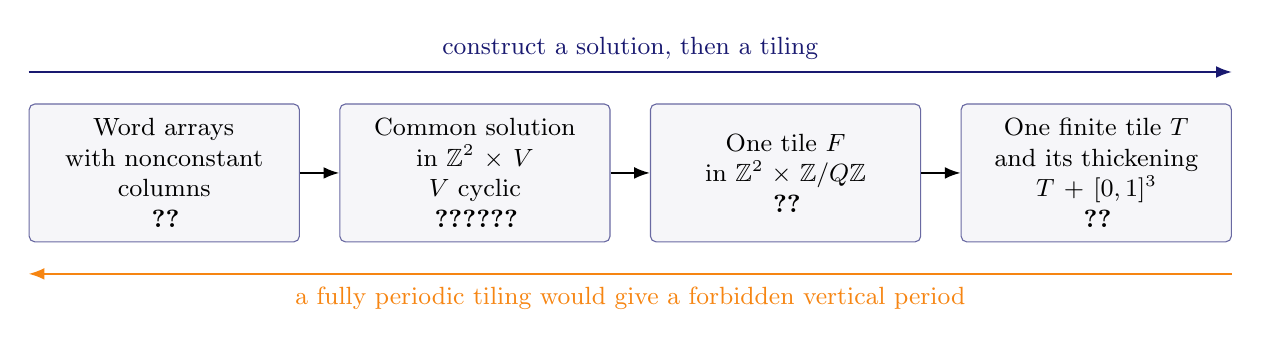
\begin{tikzpicture}[
  every node/.style={font=\small,align=center},
  stage/.style={draw=MidnightBlue!65,fill=MidnightBlue!4,
    rounded corners=2pt,text width=3.15cm,minimum height=1.75cm,inner sep=4pt},
  route/.style={-{Latex[length=2mm]},line width=.7pt}
]
\node[stage] (word) {Word arrays\\with nonconstant\\columns\\\cref{sec:word}};
\node[stage,right=5mm of word] (system) {Common solution\\in $\Z^2\times V$\\$V$ cyclic\\\cref{sec:encoding,sec:activation,sec:model}};
\node[stage,right=5mm of system] (stack) {One tile $F$\\in $\Z^2\times\Zmod Q$\\\cref{sec:stacking}};
\node[stage,right=5mm of stack] (space) {One finite tile $T$\\and its thickening\\$T+[0,1]^3$\\\cref{sec:geometry}};
\draw[route] (word) -- (system);
\draw[route] (system) -- (stack);
\draw[route] (stack) -- (space);
\draw[route,MidnightBlue] ([yshift=4mm]word.north west) --
  node[above=1pt] {construct a solution, then a tiling}
  ([yshift=4mm]space.north east);
\draw[route,BurntOrange] ([yshift=-4mm]space.south east) --
  node[below=1pt] {a fully periodic tiling would give a forbidden vertical period}
  ([yshift=-4mm]word.south west);
\end{tikzpicture}
\caption{The two directions of the proof. The construction proceeds to
 the right, starting from the explicit last-nonzero-digit array in
 \cref{word:model}. To exclude full periodicity, any hypothetical periodic tiling
 is decoded in the reverse direction, producing a line-rule array
 with nonconstant columns and a vertical period. Every tiling equation at the
 second stage uses the same translation set, and the last stage uses
 the same $T$ in both the discrete and Euclidean assertions.}
\label{fig:proof-route}
\end{figure}


\section{A word rule with no vertical period}
\label{sec:word}

We begin with a finite word constraint whose solutions on an infinite strip
cannot have a vertical period if every column is nonconstant.  The constraint
is the two-digit $p$-adic Sudoku rule of
\citet[Definition~4.5]{GTUndecidable}.  The affine-square and rescaling
arguments below follow the framework of
\citet[Theorem~4.7, Lemma~4.8, and Section~4.2]{GTUndecidable}; we give the
complete argument for the particular obstruction needed here.

Fix a prime $p>200$, and set
\[
    N=p^2,\qquad \Sigma=\Fp^\times,
    \qquad I=\{0,1,\ldots,N-1\}.
\]
When an integer occurs in an expression over $\Fp$, its residue modulo $p$
is understood.

\begin{definition}[Allowed words and the line rule]
\label{word:definition}
A word $w\colon I\to\Sigma$ is \emph{allowed} if there are integers $a,b$,
not both divisible by $p$, such that, for every $n\in I$,
\[
 w(n)=
 \begin{cases}
   an+b\pmod p, & p\nmid an+b,\\[2pt]
   (an+b)/p\pmod p, & p\mid an+b\text{ and }p^2\nmid an+b.
 \end{cases}
\]
At indices with $p^2\mid an+b$, the value may be any member of $\Sigma$.
An array $W\colon I\times\Z\to\Sigma$ satisfies the \emph{line rule} if
\[
    n\longmapsto W(n,dn+e)
\]
is an allowed word for every $d,e\in\Z$.
A \emph{positive vertical period} of $W$ is an integer $M>0$ such that
$W(n,m+M)=W(n,m)$ for all $(n,m)\in I\times\Z$.
\end{definition}

The allowed-word constraint depends only on the residues of $a,b$ modulo
$p^2$.  Indeed, these residues determine the divisibility alternatives
and each of the prescribed values.  In particular, it is a finite
constraint on words over the finite alphabet $\Sigma$.

For every allowed word, reduction of a witnessing pair gives a nonzero
affine form $\ell(n)=\bar a n+\bar b$ over $\Fp$.  The word agrees with
$\ell$ wherever $\ell\ne0$.  A nonzero affine form has at most one zero
residue class, so there are at most $N/p=p$ exceptional indices on $I$.
Here and below, ``nonzero affine form'' means that its coefficients are
not all zero; a nonzero constant form is permitted.

\begin{lemma}[Global affine approximation]
\label{word:affine}
If $W$ satisfies the line rule, there are $A,B,C\in\Fp$, not all zero,
such that
\[
    W(n,m)=An+Bm+C
    \quad\text{whenever }An+Bm+C\ne0.
\]
\end{lemma}

\begin{proof}
For each line $m=dn+e$ with $d\in\{-1,0,1\}$, choose the nonzero affine
form $\ell_{d,e}(n)$ supplied by an allowed-word witness.  Call an index on
that line exceptional when $\ell_{d,e}(n)=0$.

First we find a consecutive $4\times4$ square containing no exceptional
cell for any of these three line directions.  In the rectangle
$I\times\{0,\ldots,K-1\}$ there are $(N-3)(K-3)$ such squares.  The
numbers of lines of slopes $0,1,-1$ meeting the rectangle are respectively
$K,K+N-1,K+N-1$.  Each line has at most $p$ exceptional cells on the
whole strip, and each cell belongs to at most $16$ candidate squares.
Consequently at most
\[
    16p(3K+2N-2)\leq16p(3K+2N)
\]
squares are excluded.  Since
\[
    N-3-48p=p^2-48p-3>0,
\]
we can choose an integer $K\geq4$ with
\[
    K>\frac{3(N-3)+32pN}{N-3-48p}.
\]
For this choice,
\[
    (N-3)(K-3)-16p(3K+2N)
      =K(N-3-48p)-3(N-3)-32pN>0.
\]
A square of the required kind therefore exists.

Write its column indices as $r,r+1,r+2,r+3$ and its row indices as
$q,q+1,q+2,q+3$.  Each row agrees on the square with an affine function
$U_m n+V_m$.  For $m=q+1,q+2$ and $n=r+1,r+2$, the second difference
along either diagonal vanishes.  Thus, for each sign,
\[
 \begin{split}
  0={}&n(U_{m+1}-2U_m+U_{m-1})
       +(V_{m+1}-2V_m+V_{m-1})\\
     &\qquad\qquad{}\pm(U_{m+1}-U_{m-1}).
 \end{split}
\]
Subtracting the identities at the two consecutive values of $n$ gives
$U_{m+1}-2U_m+U_{m-1}=0$.  Subtracting the two signs gives
$U_{m+1}=U_{m-1}$, because $2\ne0$ in $\Fp$.  Together these imply
$U_{m-1}=U_m=U_{m+1}$.  The two overlapping triples show that all four
row slopes have a common value $A$.  The remaining identities say that
the four intercepts have zero second differences, so they have the form
$V_m=Bm+C$.  Therefore the form
\[
    H(n,m)=An+Bm+C
\]
agrees with $W$ on the square.  It is not the zero form, because every
entry of $W$ lies in $\Sigma$.

Call a cell \emph{good} if either $H(n,m)=0$ or $W(n,m)=H(n,m)$.  We claim
that four consecutive good cells on a line of slope $0,1$, or $-1$ make
the entire line good.  The restriction of $H$ to that line is an affine
form in $n$.  If it is identically zero, the claim follows from the
definition of goodness.  Otherwise, it and the chosen form
$\ell_{d,e}$ each have at most one zero among the four indices, which
are distinct modulo $p$.  At least two of the four indices remain where
both forms are nonzero.  At these indices, goodness and the word rule
identify both forms with $W$.  Two distinct residues determine an
affine form, so the two forms are equal.  Wherever this common form is
nonzero the word rule gives $W=H$, and its zeros are good by definition.
This proves the claim.

Applying the claim to the four square rows makes those entire rows good.
To adjoin a row immediately above a block of four good rows, consider
its cell in column $n$.  At least one of
\[
    n+4\leq N-1\qquad\text{or}\qquad n-4\geq0
\]
holds, since $N\geq8$.  Choose $\varepsilon\in\{-1,1\}$ so that the four
columns $n+\varepsilon,n+2\varepsilon,n+3\varepsilon,n+4\varepsilon$
are in $I$.  If the new row has index $m$, the cells
\[
    (n+j\varepsilon,m-j),\qquad 1\leq j\leq4,
\]
are four consecutive good cells on a diagonal through $(n,m)$.  The
claim makes $(n,m)$ good.  For a row immediately below a block of four
good rows, use $(n+j\varepsilon,m+j)$ instead.  These formulas include
both edge columns of the strip.  Successively adjoining rows in both
directions makes every cell good, proving the lemma.
\end{proof}

\begin{lemma}[Vertical nondegeneracy]
\label{word:vertical}
Let $H(n,m)=An+Bm+C$ be any affine form supplied by
\cref{word:affine}.  Every column of $W$ is nonconstant if and only if
$B\ne0$.  In that case every positive vertical period of $W$ is
divisible by $p$.
\end{lemma}

\begin{proof}
If $B=0$, then $An+C$ is not identically zero.  Some $n\in\{0,\ldots,p-1\}$
therefore has $An+C\ne0$, and the entire column at that $n$ has the
constant value $An+C$.  Conversely, if $B\ne0$, then for any fixed $n$
the form $An+Bm+C$ runs through $\Fp$ as $m$ runs through a complete
residue system modulo $p$.  At its $p-1$ nonzero values, the entries of
$W$ equal those values.  Thus every column takes every symbol of
$\Sigma$, and in particular is nonconstant.

Suppose now that $M>0$ satisfies $W(n,m+M)=W(n,m)$ for every $(n,m)$.
For a fixed $n$, choose $m$ so that both $H(n,m)$ and $H(n,m+M)$ are
nonzero.  There are at most two excluded residue classes, so this is
possible.  Equality of the two entries gives
\[
    BM=H(n,m+M)-H(n,m)=0\quad\text{in }\Fp.
\]
Since $B\ne0$, this implies $p\mid M$.
\end{proof}

\begin{proposition}[The vertical-period obstruction]
\label{word:obstruction}
There is no array $W\colon I\times\Z\to\Sigma$ satisfying the line rule,
having every column nonconstant, and having a positive vertical period.
\end{proposition}

\begin{proof}
Suppose otherwise, and choose the smallest positive integer $M$ that
occurs as a vertical period of any such array.  Choose an array with
period $M$ and an affine approximation $An+Bm+C$.  By
\cref{word:vertical}, $B\ne0$ and $p\mid M$.

Choose integers $u,v$ with $A+Bu=C+Bv=0$ in $\Fp$, and replace $W$ by
\[
    \widetilde W(n,m)=W(n,m+un+v).
\]
On a line of slope $d$ and intercept $e$, this samples the original
line of slope $d+u$ and intercept $e+v$, so the line rule is preserved.
Each column is simply translated in its row coordinate; hence column
nonconstancy and the set of vertical periods are preserved.  The new
affine approximation is $Bm$.  Rename this normalized array $W$.

Define
\[
    W_1(n,m)=W(n,pm).
\]
This array also satisfies the line rule: its line with slope $d$ and
intercept $e$ is the old line with slope $pd$ and intercept $pe$.
By \cref{word:affine}, it has a nonzero affine approximation
$H_1(n,m)=A_1n+B_1m+C_1$.  We next prove $B_1\ne0$, which is the step
needed to retain column nonconstancy under this rescaling.

If $B_1=0$, choose $0\leq n_0<p$ with
$c=A_1n_0+C_1\ne0$.  Apply the word rule for $W$ to the line
$m=n-n_0$, and let $a,b$ be a witnessing pair.  Away from the at most
two zero residue classes of $\bar a n+\bar b$ and $B(n-n_0)$, both
forms equal the array entry on that line.  Since $p-2\geq2$, they agree
at two distinct residues and therefore are the same affine form.  In
particular,
\[
    a\equiv B\pmod p,\qquad b\equiv-Bn_0\pmod p.
\]
It follows that $p\mid an_0+b$ and $p\nmid a$.

For $0\leq k<p$, put $n=n_0+pk$; all these indices lie in $I$,
including the largest possible value $p^2-1$.  At the corresponding
point of the line, the entry is
\[
    W(n_0+pk,pk)=W_1(n_0+pk,k)=c,
\]
where the last equality follows from the nonzero value
$H_1(n_0+pk,k)=c$.  On the other hand,
\[
    a(n_0+pk)+b
       =p\left(\frac{an_0+b}{p}+ak\right).
\]
Whenever the parenthesized expression is nonzero modulo $p$, the second
case of the allowed-word rule forces this entry to equal
\[
    \frac{an_0+b}{p}+ak\pmod p.
\]
As $k$ runs from $0$ to $p-1$, these residues run through all of $\Fp$,
because $p\nmid a$.  Thus $p-1$ of the entries are forced to take the
$p-1$ distinct nonzero values, contradicting their common value $c$.
The remaining index, where the rule prescribes no value, is not needed
for this contradiction.

We have proved $B_1\ne0$, so every column of $W_1$ is nonconstant by
\cref{word:vertical}.  But $M/p$ is a positive vertical period of $W_1$,
since
\[
    W_1(n,m+M/p)=W(n,pm+M)=W(n,pm)=W_1(n,m).
\]
This contradicts the choice of $M$.
\end{proof}

\begin{lemma}[A model for the line rule]
\label{word:model}
For $t\in\Z\setminus\{0\}$, let $\operatorname{ord}_p(t)$ be the
largest nonnegative integer $r$ for which $p^r\mid t$, and define
\[
    f(t)=\frac{t}{p^{\operatorname{ord}_p(t)}}\pmod p,
    \qquad f(0)=1.
\]
Then $f\colon\Z\to\Sigma$, and the array $W(n,m)=f(m)$ satisfies the
line rule and has every column nonconstant.
\end{lemma}

\begin{proof}
The definition gives a nonzero residue for every nonzero integer,
including negative integers.  For every $r\geq0$ and $t\in\Z$ we have
$f(p^rt)=f(t)$; this also holds at $t=0$ by definition.

Fix integers $d,e$.  If $(d,e)\ne(0,0)$, let $r$ be the largest integer
such that $p^r$ divides both coefficients, and write $d=p^ra$, $e=p^rb$.
The pair $a,b$ is not both divisible by $p$, and
\[
    f(dn+e)=f(an+b)\qquad(n\in I).
\]
When $an+b$ has $p$-adic order zero or one, this is exactly the
respective value prescribed by the allowed-word rule.  When
$p^2\mid an+b$, including $an+b=0$, the rule leaves the value
unrestricted.  Thus $a,b$ witness that the word is allowed.  If
$(d,e)=(0,0)$, the word is constantly $1$ and has witness $a=0,b=1$.
Finally $f(1)=1$ and $f(2)=2$, so every column is nonconstant.
\end{proof}

For the encoding that follows, parametrize the lines by
$x=(x_1,x_2)\in\Z^2$ and write
\begin{equation}
\label{word:line-maps}
    L_n(x)=x_2+nx_1,\qquad u_n=(1,-n)\qquad(n\in I).
\end{equation}
The map $L_n\colon\Z^2\to\Z$ is surjective and its kernel is generated
by $u_n$: the equation $x_2+nx_1=0$ is equivalent to
$x=x_1(1,-n)$.  The model supplies the allowed word
$\bigl(f(L_n(x))\bigr)_{n\in I}$ at every $x$.  Moreover, if
$x_1\equiv0$ and $x_2\equiv t\pmod p$ for $t\in\{1,2\}$, every entry
of this word equals $t$.  Indeed, every $L_n(x)$ then has the nonzero
residue $t$, so its last nonzero digit is $t$.

\section{Encoding symbols in a cyclic finite coordinate}
\label{sec:encoding}

We now express the word constraints by finitely many translational tiling
equations on a common unknown set.  A symbol will be represented by the
dependence of a function on one of its input digits.  The present section
constructs tests forbidding specified simultaneous dependences; the next
section will force enough dependence to obtain an array. Encoding
functional constraints by tiling equations is developed in
\citet[Sections~4--8]{GTTwoTiles} and
\citet[Theorem~4.1]{GTPeriodic}. The issue here is to carry out the
required tests with a cyclic finite factor; the graph, dependence,
and cycle constructions below supply their exact local forms.

\subsection{Channels and the ambient group}

Retain the prime $p>200$, the width $N=p^2$, and the alphabet
$\Sigma=\Fp^\times$ from the preceding section.  Recall the line maps
$L_n(x)=x_2+nx_1$ and their kernel generators $u_n=(1,-n)$ from
\eqref{word:line-maps}.  The set of
\emph{channels} is
\[
 \mathcal I=\{0,\ldots,N-1\}\sqcup\{\eta_1,\eta_2\}.
\]
The first $N$ channels are ordinary; the last two are seeds.  Their input
digit labels are $J_n=\Sigma$ and $J_{\eta_t}=\{*\}$, respectively.
The seeds will eventually require the ordinary channels to display the
constant words $1$ and $2$ at some points.  Set
\[
 S=(\Zmod{p^2})^2,\qquad s(x)=x\bmod p^2,\qquad D=\abs{S}=p^4.
\]
Here $S$ records residues of the horizontal variable $x$.

For each $i\in\mathcal I$, choose primes $a_i,b_i$ and put
$P_i=\Zmod{a_i}\times\Zmod{b_i}$.  Require
\[
 a_{\eta_1}=2,\qquad a_{\eta_2}=3,\qquad
 b_{\eta_1},b_{\eta_2}>D,
\]
and choose all the $a_i,b_i$ to be distinct and different from $p$.
For each $j\in J_i$, choose a further prime $r_{ij}$, with all these
primes distinct and disjoint from the previous choices, such that
\begin{equation}
 r_{ij}=A_{ij}a_i+B_{ij}b_i,
 \qquad A_{ij},B_{ij}\in\Z_{\geq0}.
 \label{enc:digit-partition}
\end{equation}
These choices are possible using only finitely many primes.  Indeed, if
$a,b$ are coprime and $r\geq(a-1)b$, choose $B\in\{0,\ldots,a-1\}$
with $Bb\equiv r\pmod a$; then $A=(r-Bb)/a$ is a nonnegative integer.
There are arbitrarily large primes outside any prescribed finite set,
so this argument applies successively to every required $r_{ij}$.

Write
\[
 r_i=\prod_{j\in J_i}r_{ij},\qquad
 K_i=\Zmod{r_i}\cong\prod_{j\in J_i}\Zmod{r_{ij}},\qquad
 K=\prod_{i\in\mathcal I}K_i,\qquad
 P=\prod_{i\in\mathcal I}P_i.
\]
The displayed identification of $K_i$ is the Chinese remainder
isomorphism, given by taking residues.  Let $U_{ij}\leq K_i$ be the
coordinate subgroup supported on the digit $j$ in this identification.
We work in
\begin{equation}
 G=\Z^2\times V,\qquad
 V=\Zmod D\times\prod_{i\in\mathcal I}
       \bigl(\Zmod{r_i^2}\times P_i\bigr).
 \label{enc:ambient}
\end{equation}
The group $V$ is cyclic.  To see this, expand each $P_i$ into its two
cyclic factors.  The orders $D$, $r_i^2$, $a_i$, and $b_i$ of all the
resulting factors are pairwise coprime.  A tuple of generators therefore
has order equal to their product, which is $\abs V$.
The residue set $S$ is not an additional factor of $V$; the coordinate
of order $D$ in \eqref{enc:ambient} is the cyclic group $\Zmod D$.

\subsection{One graph and freely chosen high coordinates}

Write an element of $G$ as
\[
 \bigl(x,z,(v_i,c_i)_{i\in\mathcal I}\bigr),\qquad
 z\in\Zmod D,\quad v_i\in\Zmod{r_i^2},\quad c_i\in P_i.
\]
Its low coordinates are $k_i=v_i\bmod r_i\in K_i$.  Let
$q_0:G\to\Z^2\times K$ be the homomorphism retaining just $(x,k)$,
and let
\[
 H_0=\ker q_0
   =\{0\}\times\Zmod D\times
       \prod_{i\in\mathcal I}
       \bigl(r_i(\Zmod{r_i^2})\times P_i\bigr).
\]
Include the tiling equation
\begin{equation}
 A\oplus H_0=G.
 \label{enc:graph}
\end{equation}
For a target point in any fibre of $q_0$, every element of $A$ in that
fibre supplies exactly one representation with a summand in $H_0$.
Consequently \eqref{enc:graph} says precisely that $A$ contains one
point above each $(x,k)$.  We may thus denote its outputs by
$c_i(x,k)$, $z(x,k)$, and $v_i(x,k)$.

For subsequent constructions it is useful to describe $v_i$ by a
sheared high coordinate $\beta_i(x,k)\in K_i$, defined by
\begin{equation}
 v_i(x,k)=x_1+[k_i-x_1]_{r_i}+r_i\beta_i(x,k)
       \quad\text{in }\Zmod{r_i^2}.
 \label{enc:shear}
\end{equation}
Here $[\cdot]_{r_i}$ is the least nonnegative representative modulo
$r_i$.  For fixed $x,k_i$, the right side is a bijection from $K_i$
onto the elements of $\Zmod{r_i^2}$ with residue $k_i$.
Thus arbitrary functions $c_i$, $\beta_i$, and $z$ specify exactly one
graph satisfying \eqref{enc:graph}.  This is a choice of coordinates
on each fibre; it does not assert a direct-product splitting of
$\Zmod{r_i^2}$ into two groups of order $r_i$.

If we add $h=(h_1,h_2)$ to $x$ and $h_1$ to $v_i$, the new low
coordinate is $k_i+h_1$.  Since
\[
 [(k_i+h_1)-(x_1+h_1)]_{r_i}=[k_i-x_1]_{r_i},
\]
this operation preserves $\beta_i$.  The identity holds for every
integer lift of $h_1$, including negative ones.

\subsection{Dependence constraints on the useful outputs}

We require exactly the following restrictions on the functions $c_i$:
\begin{equation}
 \begin{aligned}
 c_n(x,k)&=\widetilde c_n(L_n(x),k_n)
       &&(0\leq n<N),\\
 c_{\eta_t}(x,k)&=\widetilde c_{\eta_t}(s(x),k_{\eta_t})
       &&(t=1,2).
 \end{aligned}
 \label{enc:dependence}
\end{equation}
The outputs $c_i$ will encode symbols; the other outputs will be used
to satisfy the activation equations.

\begin{lemma}\label{enc:invariance}
Fix a channel $i$ and a shift $\sigma\in\Z^2\times K$.
There is a finite nonempty tile $F_{i,\sigma}\subset G$ such that,
for every graph satisfying \eqref{enc:graph},
\[
 A\oplus F_{i,\sigma}=G
 \quad\Longleftrightarrow\quad
 c_i(b-\sigma)=c_i(b)\text{ for every }b\in\Z^2\times K.
\]
This equation imposes no restriction on the graph's other outputs.
\end{lemma}

\begin{proof}
Choose any lift $g\in G$ of $\sigma$ with $c_i$-coordinate zero, and
partition $H_0$ into
\[
 E_0^{(i)}=\{h\in H_0:c_i(h)=0\},\qquad
 E_{\ne0}^{(i)}=H_0\setminus E_0^{(i)}.
\]
Set
\[
 F_{i,\sigma}=E_{\ne0}^{(i)}\sqcup(g+E_0^{(i)}).
\]
The union is disjoint because its two parts have, respectively,
nonzero and zero $c_i$-coordinates.  Fix a target base $b$.
The unique graph point above $b$, together with $E_{\ne0}^{(i)}$,
covers exactly those points in that fibre whose $c_i$-coordinate
differs from $c_i(b)$, once each.  The graph point above $b-\sigma$,
together with $g+E_0^{(i)}$, covers exactly the points whose
$c_i$-coordinate is $c_i(b-\sigma)$, once each.
In both assertions, every choice of the other outputs and high
coordinates is attained exactly once, since those offsets range
freely in $E_0^{(i)}$.  The two contributions partition the target
fibre precisely when the displayed equality of useful outputs holds.
\end{proof}

Apply \cref{enc:invariance}, for each $i$, to a generator of every
$K_\ell$ with $\ell\ne i$, keeping all other base coordinates fixed.
This removes dependence on the other low inputs.  For an ordinary
channel $n$, also apply it to the horizontal shift $u_n$ with zero
low-coordinate shift.  Since $\ker L_n=\Z u_n$, the remaining
dependence on $x$ factors through $L_n(x)$.  For each seed use instead
the two horizontal shifts $(p^2,0)$ and $(0,p^2)$, again with zero
low-coordinate shift.  These give precisely dependence on $s(x)$.
There are only finitely many such generators and tiles, and their
equations are equivalent to \eqref{enc:dependence}.  In particular,
they leave all the functions $\beta_i$ and $z$ unrestricted.

For a graph with these dependences, write
$g_{i,x}:K_i\to P_i$ for its useful output at $x$.  Define its
\emph{active labels} by
\[
 \mathcal A_i(x)=
 \bigl\{j\in J_i:\text{there exist }w,w'\in K_i
   \text{ with }w-w'\in U_{ij}
   \text{ and }g_{i,x}(w)\ne g_{i,x}(w')\bigr\}.
\]
Thus a label is inactive exactly when changing that digit never
changes the output.  For ordinary $n$, the set $\mathcal A_n(x)$
depends only on $L_n(x)$; for a seed it depends only on $s(x)$.
A function independent of every digit is constant, since one can
pass between any two inputs by changing one digit at a time.
At this stage the active sets are allowed to be empty.

\subsection{A cycle test for simultaneous activity}

\begin{lemma}[Exclusion of simultaneous activity]\label{enc:exclusion}
Let $C=(i_1,\ldots,i_t)$ be a nonempty cyclically ordered list of
distinct channels, and choose a label $j(i)\in J_i$ for each $i\in C$.
There is a finite family of finite nonempty tiles such that a graph
satisfying \eqref{enc:dependence} tiles with every member of this
family if and only if, at every $x\in\Z^2$, at least one of the
chosen labels $j(i)$ is inactive.
\end{lemma}

\begin{proof}
For each $i\in C$, let $\operatorname{prev}(i)$ denote the preceding
channel in the cycle.  Choose arbitrary maps
\[
 d_i:P_{\operatorname{prev}(i)}\longrightarrow U_{i,j(i)}.
\]
For $e=(e_i)_{i\in\mathcal I}\in P$, put
\[
 d_i[e]=
 \begin{cases}
  d_i(e_{\operatorname{prev}(i)})&i\in C,\\
  0&i\notin C.
 \end{cases}
\]
Include a tile for every joint choice $d=(d_i)_{i\in C}$, namely
\begin{equation}
 F_d=\left\{
 \bigl(0,\zeta,(\upsilon_i,e_i)_{i\in\mathcal I}\bigr):
 \begin{array}{l}
 e\in P,\quad \zeta\in\Zmod D,\\
 \upsilon_i\in\Zmod{r_i^2},\quad
 \upsilon_i\bmod r_i=d_i[e]\quad(i\in\mathcal I)
 \end{array}
 \right\}.
 \label{enc:cycle-tile}
\end{equation}
This is an ordinary set: distinct $e$ give distinct useful-output
offsets, and every choice of $\zeta$ and the lifts $\upsilon_i$
occurs once.  Both the tile and the family of all maps $d$ are finite.

Fix a target base $(x,k)$.  For a fixed $e$, a representation using
\eqref{enc:cycle-tile} must start at the graph point over
$(x,(k_i-d_i[e])_i)$.  The useful outputs of the target are then
\begin{equation}
 \Phi_{x,k,d}(e)
   =\bigl(e_i+g_{i,x}(k_i-d_i[e])\bigr)_{i\in\mathcal I}.
 \label{enc:permutation}
\end{equation}
For any prescribed remaining coordinates of the target, the offsets
$\zeta$ and $\upsilon_i$ are uniquely determined: each low residue is
already correct, and all its lifts occur in the tile.
Hence $A\oplus F_d=G$ holds exactly when \eqref{enc:permutation} is a
permutation of $P$ for every $(x,k)$.  This criterion is independent
of the graph's high outputs and its $z$-output.

Suppose some $j(i_0)$ is inactive at $x$.  Then the $i_0$-component
of \eqref{enc:permutation} is $e_{i_0}+g_{i_0,x}(k_{i_0})$,
independent of the preceding component of $e$.
From any target useful-output tuple, we can therefore recover
$e_{i_0}$ uniquely.  The next equation around the cycle then recovers
the next component, and continuing recovers all components on $C$.
The starting equation remains satisfied because it never depended
on the preceding component.  Off the cycle, each equation is just a
fixed translation and recovers its component separately.  This gives
a unique preimage for every target, for all $k$ and all maps $d$.

Conversely, suppose every chosen label is active at some $x$.
For each $i\in C$ choose $w_i,w_i'\in K_i$ such that
\[
 w_i-w_i'\in U_{i,j(i)},\qquad
 \varepsilon_i:=g_{i,x}(w_i)-g_{i,x}(w_i')\ne0.
\]
Set $k_i=w_i$ on the cycle, and choose the other $k_i$ arbitrarily.
Extend $\varepsilon$ by zero off $C$ to an element of $P$.
For each $i\in C$, choose a map with
\[
 d_i(0)=0,\qquad
 d_i(\varepsilon_{\operatorname{prev}(i)})=w_i-w_i'.
\]
The two specified arguments are distinct, so these prescriptions
extend to maps on the whole domain.  They are among the maps tested
in the finite family.  At this base, the distinct inputs $0$ and
$\varepsilon$ have the same image under \eqref{enc:permutation}:
on $C$ their outputs are respectively $g_{i,x}(w_i)$ and
$\varepsilon_i+g_{i,x}(w_i')$, and off $C$ they coincide as well.
The permutation condition fails.  This proves both directions.
\end{proof}

Let $\mathcal W\subseteq\Sigma^N$ be the finite set of allowed words
from the word rule.  We impose the following specific instances of
\cref{enc:exclusion}:
\begin{enumerate}
 \item For every $w\in\Sigma^N\setminus\mathcal W$, use the cycle
 $(0,1,\ldots,N-1)$ with label $j(n)=w(n)$.
 \item For each $t\in\{1,2\}$, each ordinary channel $n$, and each
 $j\in\Sigma\setminus\{t\}$, use the two-channel cycle
 $(\eta_t,n)$ with labels $*$ and $j$.
\end{enumerate}
All these instances form a finite family.  Their precise consequences
are
\begin{equation}
 \prod_{n=0}^{N-1}\mathcal A_n(x)\subseteq\mathcal W,
 \qquad
 *\in\mathcal A_{\eta_t}(x)
   \ \Longrightarrow\ 
   \mathcal A_n(x)\subseteq\{t\}\quad(0\leq n<N).
 \label{enc:word-exclusions}
\end{equation}
The first product is identified with a set of words in the natural
order of the channels.  These statements also hold when some active
sets are empty.  The activation tiles constructed next will ensure
that every ordinary active set is nonempty at every point and that
each seed is active somewhere.

Every tile constructed in this section is a finite nonempty subset
of $G$.  As a check on the fibre counts, all have cardinality
\[
 \abs{H_0}=D\prod_{i\in\mathcal I}r_i\abs{P_i}:
\]
the dependence tiles partition a copy of $H_0$ into two shifted
pieces, while each cycle tile has $\abs P$ choices of $e$, $D$
choices of $\zeta$, and $r_i$ choices of each lift $\upsilon_i$.

\section{Forcing activity and excluding full periodicity}
\label{sec:activation}

The exclusion equations constrain which labels can be active together.
We now add one finite tile for each channel to ensure that every ordinary
channel is active at every point, and that each seed is active somewhere.
Throughout this section, we retain the groups and coordinates of
\cref{sec:encoding}.  In particular, the useful output of channel $i$ is
$c_i\in P_i=\Zmod{a_i}\times\Zmod{b_i}$, its low input is $k_i\in K_i$,
and its sheared high coordinate is $\beta_i\in K_i$.

\subsection{A shift list with two fibre orderings}

The shift list will serve two purposes: its nonuniform multiplicities
will force activity, while its uniform counts in each coordinate will
permit the explicit common solution in \cref{sec:model}.

Fix a channel $i$.  For $e\in P_i$, let $\mathbf 1_{\{e\}}$ denote the
indicator of the singleton $\{e\}$, and define the integer-valued functions
\[
 \omega_i
 =\mathbf 1_{\{(0,0)\}}-\mathbf 1_{\{(1,0)\}}
  -\mathbf 1_{\{(0,1)\}}+\mathbf 1_{\{(1,1)\}},
 \qquad
 \mu_i=1+\omega_i
 \quad\text{on }P_i.
\]
Here $1$ denotes the constant function.  The function $\mu_i$ has values
two at $(0,0)$ and $(1,1)$, zero at $(1,0)$ and $(0,1)$, and one elsewhere.
It is therefore a nonnegative, nonconstant multiplicity function.
Its total mass is $a_i b_i$, and its marginals are uniform:
\[
 \sum_{\alpha\in\Zmod{a_i}}\mu_i(\alpha,\xi)=a_i
 \quad(\xi\in\Zmod{b_i}),
 \qquad
 \sum_{\xi\in\Zmod{b_i}}\mu_i(\alpha,\xi)=b_i
 \quad(\alpha\in\Zmod{a_i}).
\]
Choose an index set $\Delta_i$ of size $a_i b_i$ and a list
$e_\delta=(e_\delta^a,e_\delta^b)\in P_i$, $\delta\in\Delta_i$, in
which each $e\in P_i$ occurs $\mu_i(e)$ times.  The following notation
for the list and its orderings is local to channel $i$.

For each $\xi$, order the $a_i$ indices with $e_\delta^b=\xi$ by an
arbitrary bijection to $\Zmod{a_i}$, and define $\rho^a(\delta)$ by
subtracting $e_\delta^a$ from that assigned value.  Independently, for
each $\alpha$, order the $b_i$ indices with $e_\delta^a=\alpha$ by a
bijection to $\Zmod{b_i}$, and subtract $e_\delta^b$ to define
$\rho^b(\delta)$.  Thus both maps in
\begin{equation}
\label{act:fibre-orderings}
\begin{aligned}
 \{\delta\in\Delta_i:e_\delta^b=\xi\}
   &\longrightarrow\Zmod{a_i},
 &\delta&\longmapsto e_\delta^a+\rho^a(\delta),\\
 \{\delta\in\Delta_i:e_\delta^a=\alpha\}
   &\longrightarrow\Zmod{b_i},
 &\delta&\longmapsto e_\delta^b+\rho^b(\delta)
\end{aligned}
\end{equation}
are bijections.  Repeated values of $e_\delta$ have distinct indices;
the orderings act on these indices.

\subsection{The activation tiles}

For a channel $\ell$, write
$R_\ell=r_\ell\Zmod{r_\ell^2}$ for the subgroup of offsets with low
coordinate zero.  It has $r_\ell$ elements.  Given $h\in\Z^2$,
$e\in P_i$, and $E\subseteq\Zmod{D}$, define a batch of offsets by
\[
\begin{split}
 \mathcal B_i(h,e;E)=
 \bigl\{\bigl(h,\zeta,(w_\ell,d_\ell)_{\ell\in\mathcal I}\bigr):
 &\ \zeta\in E,\quad
 w_i=h_1\pmod{r_i^2},\quad d_i=e,\\[-2pt]
 &\ w_\ell\in R_\ell,\quad d_\ell\in P_\ell
       \text{ for every }\ell\ne i\bigr\}.
\end{split}
\]
Every combination of the freely varied coordinates occurs once in this
set.

For an ordinary channel $i\in\{0,\ldots,N-1\}$ and each pair
$(l,\delta)\in K_i\times\Delta_i$, choose an integer multiple
$h=h^{(i)}_{l,\delta}$ of $u_i=(1,-i)$ such that
\begin{equation}
\label{act:ordinary-crt}
 h_1\equiv l\pmod{r_i},\qquad
 h_1\equiv\rho^a(\delta)\pmod{a_i},\qquad
 h_1\equiv\rho^b(\delta)\pmod{b_i}.
\end{equation}
The moduli are pairwise coprime, so the Chinese remainder theorem gives
infinitely many choices of $h_1$.  Choose these horizontal offsets
distinctly for the different pairs $(l,\delta)$, and set
\[
 F_i^{\mathrm{act}}
 =\bigcup_{(l,\delta)\in K_i\times\Delta_i}
    \mathcal B_i\bigl(h^{(i)}_{l,\delta},e_\delta;\Zmod{D}\bigr).
\]
The restriction $h\in\Z u_i$ gives $L_i(x-h)=L_i(x)$ for every $x$.

For a seed $i\in\{\eta_1,\eta_2\}$, let $i'$ denote the other seed.
For every $(l,\delta,\tau)\in K_i\times\Delta_i\times S$, choose
$h=h^{(i)}_{l,\delta,\tau}\in\Z^2$ satisfying
\cref{act:ordinary-crt} and the additional conditions
\begin{equation}
\label{act:seed-crt}
 s(h)=\tau,\qquad h_1\equiv0\pmod{a_{i'}}.
\end{equation}
There is no slope restriction in this case.  Writing
$\tau=(\tau_1,\tau_2)\in(\Zmod{p^2})^2$, the first coordinate is
prescribed modulo the pairwise coprime integers
$r_i,a_i,b_i,p^2,a_{i'}$, while the second coordinate only needs to
satisfy $h_2\equiv\tau_2\pmod{p^2}$.  Again there are infinitely many
choices, so take all horizontal offsets within this seed tile to be
distinct.  Define
\[
 F_i^{\mathrm{act}}
 =\bigcup_{(l,\delta,\tau)\in K_i\times\Delta_i\times S}
    \mathcal B_i\bigl(h^{(i)}_{l,\delta,\tau},e_\delta;\{0\}\bigr).
\]
Thus an ordinary batch varies the $z$-offset freely, whereas a seed batch
has $z$-offset zero.  The congruence involving $a_{i'}$ will allow both
seed tests to hold with one common $z$-output in the construction of
\cref{model:system}.

All unions just defined are disjoint unions of finite sets, because
different batches have different horizontal offsets.  In particular,
the repeated entries of the auxiliary shift list do not introduce
weighted tile elements.  These tiles are nonempty, and direct counting
gives, for every channel $i$,
\[
 \abs{F_i^{\mathrm{act}}}
   =D\prod_{\ell\in\mathcal I}r_\ell\abs{P_\ell}
   =\abs{H_0}.
\]
We add the equations $A\oplus F_i^{\mathrm{act}}=G$ to the graph,
dependence, and exclusion equations.

\subsection{Exact coverage in a fibre}

\begin{lemma}[Activation fibre criterion]
\label{act:fibre-criterion}
Suppose $A\oplus H_0=G$, so that $A$ is a graph over $(x,k)$.
For a target base point $(x,k)$ and a batch with horizontal offset $h$,
write
\begin{equation}
\label{act:source-base}
 x'=x-h,\qquad k_i'=k_i-l,\qquad k_\ell'=k_\ell\quad(\ell\ne i).
\end{equation}
For an ordinary channel $i$, the equation
$A\oplus F_i^{\mathrm{act}}=G$ holds if and only if, at every target
base point, the map
\begin{equation}
\label{act:ordinary-map}
 (l,\delta)\longmapsto
 \bigl(c_i(x',k')+e_\delta,\,\beta_i(x',k')\bigr)
\end{equation}
is a bijection from $K_i\times\Delta_i$ to $P_i\times K_i$.
For a seed $i$, the corresponding necessary and sufficient condition is
that, at every target base point,
\begin{equation}
\label{act:seed-map}
 (l,\delta,\tau)\longmapsto
 \bigl(c_i(x',k')+e_\delta,\,\beta_i(x',k'),\,z(x',k')\bigr)
\end{equation}
be a bijection from $K_i\times\Delta_i\times S$ to
$P_i\times K_i\times\Zmod{D}$.
\end{lemma}

\begin{proof}
Fix a target base point and a batch.  Every offset in that batch has the
same horizontal and low coordinates, so the graph equation supplies
exactly one possible source point of $A$: the point above the base in
\eqref{act:source-base}.  The $i$th low-coordinate shift is $l$ because
$h_1\equiv l\pmod{r_i}$.  Since $x'_1=x_1-h_1$, we have
\[
 [k_i'-x'_1]_{r_i}=[k_i-x_1]_{r_i}.
\]
Consequently the shear formula \eqref{enc:shear} gives
\[
 v_i(x',k')+h_1
   =x_1+[k_i-x_1]_{r_i}+r_i\beta_i(x',k')
   \quad\text{in }\Zmod{r_i^2}.
\]
Thus the offset preserves the sheared high coordinate $\beta_i$ exactly,
and the target useful output is $c_i(x',k')+e_\delta$.

For every $\ell\ne i$, adding the freely chosen element of $R_\ell$
fills the entire high-coordinate fibre with low coordinate $k_\ell$
once.  Independently, adding the freely chosen element of $P_\ell$
fills that useful-output coordinate once.  In an ordinary batch the
$z$-coordinate is also filled once; in a seed batch it remains equal
to $z(x',k')$.  Hence each batch covers exactly the part of the target
fibre specified by its tuple in \cref{act:ordinary-map} or
\cref{act:seed-map}, with one representation for every choice of the
remaining coordinates.  Distinct batches correspond to distinct tile
elements, so exact coverage by the whole tile is equivalent to every
specified tuple occurring once.  This is precisely the asserted
bijection condition.
\end{proof}

In particular, exact coverage forces every value of the target $c_i$
to occur $r_i$ times among the ordinary batches, or $D r_i$ times
among the seed batches.  These necessary marginal counts already force
the activity we need.

\subsection{Every required channel is active}

\begin{lemma}[Ordinary activation]
\label{act:ordinary}
Every ordinary channel has at least one active label at every
$x\in\Z^2$ in any common solution of the equations specified so far.
\end{lemma}

\begin{proof}
Suppose channel $i$ has no active label at some $x$.  A function on the
finite product $K_i=\prod_{j\in J_i}\Zmod{r_{ij}}$ that is independent
of every digit is constant: any two inputs can be joined by changing
one digit at a time.  Thus $g_{i,x}$ has a constant value $c_0\in P_i$.
By the dependence condition \eqref{enc:dependence} and the equality
$L_i(x-h)=L_i(x)$, every source in the activation test at $(x,k)$ has
$c_i(x',k')=c_0$.  For each $\delta$ there are $r_i$ choices of $l$.
The number of batches giving any target value $c\in P_i$ is therefore
\[
 r_i\mu_i(c-c_0).
\]
The fibre criterion requires this number to be $r_i$ for every $c$.
That is impossible because $\mu_i$ is not constant.
\end{proof}

\begin{lemma}[Seed activation]
\label{act:seed}
Each of the two seeds has its label active at some point of $\Z^2$
in any common solution of the equations specified so far.
\end{lemma}

\begin{proof}
Fix a seed $i$ and suppose it is nowhere active.  The dependence
condition and the absence of activity give a function $q:S\to P_i$
such that $c_i(x,k)=q(s(x))$ for every base point.  Define its
nonnegative integer histogram by
\[
 Q(\alpha,\xi)
 =\abs{\{s\in S:q(s)=(\alpha,\xi)\}},
 \qquad
 \sum_{(\alpha,\xi)\in P_i}Q(\alpha,\xi)=D.
\]
At any target base point and for a fixed $\delta$, the source pairs
\[
 (s(x'),k_i')=(s(x)-\tau,k_i-l)
\]
run once through $S\times K_i$ as $(\tau,l)$ varies.  Thus the
number of seed batches with useful output $c\in P_i$ is
$r_i\sum_{\delta\in\Delta_i}Q(c-e_\delta)$.  The necessary marginal
count from \cref{act:fibre-criterion}, divided by $r_i$, yields
\[
 (Q*\mu_i)(c)=D\qquad(c\in P_i),
\]
where $(Q*\mu_i)(c)=\sum_{e\in P_i}\mu_i(e)Q(c-e)$ is convolution
on the finite group $P_i$.  Convolution with the constant function
$1$ already equals $D$, so $Q*\omega_i=0$.  Written out, this says
\begin{equation}
\label{act:mixed-difference}
 Q(\alpha,\xi)-Q(\alpha-1,\xi)
 -Q(\alpha,\xi-1)+Q(\alpha-1,\xi-1)=0.
\end{equation}

We spell out the integer and positivity consequences of this identity.
For each $\alpha$, the difference
$Q(\alpha,\xi)-Q(\alpha-1,\xi)$ is independent of $\xi$, because
successive differences in the second coordinate vanish.  Summing such
differences along the cyclic first coordinate shows that, for any
$\alpha_0$,
\[
 Q(\alpha,\xi)-Q(\alpha_0,\xi)
   =Q(\alpha,0)-Q(\alpha_0,0).
\]
Choose $\alpha_0$ to minimize $Q(\alpha,0)$, and put
\[
 u(\alpha)=Q(\alpha,0)-Q(\alpha_0,0),
 \qquad v(\xi)=Q(\alpha_0,\xi).
\]
Both functions take nonnegative integer values, and
$Q(\alpha,\xi)=u(\alpha)+v(\xi)$.  Summing gives
\[
 D=b_i\sum_{\alpha\in\Zmod{a_i}}u(\alpha)
     +a_i\sum_{\xi\in\Zmod{b_i}}v(\xi).
\]
Since $b_i>D$ and both sums are nonnegative integers, the first sum
must vanish.  It follows that $a_i$ divides $D=p^4$.  But the two
seed values of $a_i$ are $2$ and $3$, whereas $p>200$ is prime.  This
contradiction proves the claim.
\end{proof}

\subsection{Extraction of the line array}

The graph, dependence, exclusion, and activation equations now form a
finite system of tiling equations in $G$.  Its solvability will be
proved in the next section.  We can already exclude all fully periodic
common solutions.

\begin{proposition}
\label{act:nonperiodic}
No common solution of this finite system is invariant under a
finite-index subgroup of $G$.
\end{proposition}

\begin{proof}
Let $A$ be any common solution.  Fix a total ordering of $\Sigma$.
For each ordinary channel $n$ and integer $m$, define
\[
 W(n,m)=\min\mathcal A_n((0,m)),
\]
where the minimum is taken in that ordering.  This is defined by
\cref{act:ordinary}.  The dependence condition implies that
$\mathcal A_n(x)$ depends only on $L_n(x)$; since $L_n(0,m)=m$, the
selected symbol at any $x$ is exactly $W(n,L_n(x))$.

For any integers $d,e$, consider $x=(d,e)$.  If the word
$(W(n,dn+e))_{0\le n<N}$ were forbidden, all its selected labels
would be active at $x$.  This contradicts the corresponding exclusion
equations, by \cref{enc:exclusion}.  Hence $W$ satisfies the line rule.

By \cref{act:seed}, for each $t\in\{1,2\}$ there is a point
$x^{(t)}$ where the label of $\eta_t$ is active.  The seed-pair
exclusions imply that $\mathcal A_n(x^{(t)})$ contains no symbol other
than $t$.  Since this set is nonempty, it equals $\{t\}$.  Therefore
\[
 W\bigl(n,L_n(x^{(1)})\bigr)=1,
 \qquad
 W\bigl(n,L_n(x^{(2)})\bigr)=2
 \quad\text{for every }0\le n<N.
\]
The two arguments in each column must be distinct, and every column
of $W$ is nonconstant.

Suppose now that $A$ is invariant under a finite-index subgroup
$\Lambda\le G$.  Consider the actual group element
\[
 e_{\mathrm v}=\bigl((0,1),0_V\bigr)\in G.
\]
Its coset has finite order in $G/\Lambda$, so some integer $M>0$
satisfies $M e_{\mathrm v}\in\Lambda$.  We thus obtain a period
with \emph{zero finite-coordinate component}:
\[
 A+\bigl((0,M),0_V\bigr)=A.
\]
Translation by this element takes the unique graph point above
$(x,k)$ to the unique graph point above $(x+(0,M),k)$ and leaves all
useful outputs unchanged.  It follows that every active-label set is
unchanged under $x\mapsto x+(0,M)$.  At $x=(0,m)$ this gives
$W(n,m+M)=W(n,m)$ for all $n,m$.
The array is therefore vertically periodic, satisfies the line rule,
and has every column nonconstant, contradicting
\cref{word:obstruction}.
\end{proof}

\section{A common solution of the tiling equations}\label{sec:model}

We now construct one graph satisfying all the equations of
\cref{sec:encoding,sec:activation}.  The useful output of each ordinary
channel will activate exactly the symbol $f(L_i(x))$ from
\cref{word:model}.  The high coordinates will record positions within
labelled blocks.  A further labelling of the horizontal residue set $S$
will let the two seed tests use a single common output $z$.

\subsection{Labelled blocks and their inverse map}

For every channel $i$ and digit $j\in J_i$, fix a partition of
$\Zmod{r_{ij}}$ into subsets of sizes $a_i$ and $b_i$, using the
nonnegative representation of $r_{ij}$ chosen in
\cref{sec:encoding}.  Label each subset of size $d\in\{a_i,b_i\}$
bijectively by $\Zmod d$.  Copy this same partition and these same labels
for every setting of the other digits in
$K_i=\prod_{j'\in J_i}\Zmod{r_{ij'}}$.  We obtain a partition
$\mathcal B_{i,j}$ of $K_i$ into labelled blocks.  A block fixes all
digits except $j$; its label records a position in its $j$-digit subset.
The blocks are subsets, not subgroups, and their labels need not respect
addition in $K_i$.

Define a map $C_{i,j}:K_i\to P_i$ and, for each integer $t$, a
permutation $T_{i,j}(t)$ of $K_i$ as follows.  If $k_i$ has label $y$ in
a block of size $d$, put
\[
 C_{i,j}(k_i)=
 \begin{cases}
 (y,0),&d=a_i,\\
 (0,y),&d=b_i.
 \end{cases}
\]
The permutation $T_{i,j}(t)$ sends this point to the point with label
$y+t$ in the same block, with addition in $\Zmod d$.
The map $C_{i,j}$ is independent
of every digit except $j$, since the partitions and labels were copied
unchanged over the other digits.  It is not independent of $j$: each
block has at least two positions with different useful outputs.

The following inverse calculation is the reason for the fibre
orderings in \cref{act:fibre-orderings}.

\begin{lemma}[Block inverse]\label{model:block-inverse}
Fix $i,j$, a target horizontal coordinate $x_1\in\Z$, and a target
low coordinate $k_i\in K_i$.  For each $(l,\delta)\in K_i\times\Delta_i$,
choose an integer $h_1(l,\delta)$ satisfying
\[
 h_1(l,\delta)\equiv l\pmod{r_i},\qquad
 h_1(l,\delta)\equiv\rho^a(\delta)\pmod{a_i},\qquad
 h_1(l,\delta)\equiv\rho^b(\delta)\pmod{b_i}.
\]
Then the map
\begin{equation}\label{model:block-map}
 (l,\delta)\longmapsto
 \left(
 C_{i,j}(k_i-l)+e_\delta,
 T_{i,j}\bigl(x_1-h_1(l,\delta)\bigr)(k_i-l)
 \right)
\end{equation}
is a bijection from $K_i\times\Delta_i$ to $P_i\times K_i$.
\end{lemma}

\begin{proof}
Fix a target $((\alpha^*,\xi^*),\beta_i^*)$.
The point $\beta_i^*$ specifies one block $B\in\mathcal B_{i,j}$ and
its label $q$.  As each $T_{i,j}(t)$ preserves its block, any preimage
must have its source $k_i'=k_i-l$ in $B$.

Suppose first that $B$ has size $a_i$.  Choose $\delta$ by the two
conditions
\begin{equation}\label{model:a-inverse}
 \begin{aligned}
 e_\delta^b&=\xi^* &&\text{in }\Zmod{b_i},\\
 e_\delta^a+\rho^a(\delta)&=\alpha^*+x_1-q
       &&\text{in }\Zmod{a_i}.
 \end{aligned}
\end{equation}
The first fibre ordering makes this choice unique.  Set
$y=\alpha^*-e_\delta^a$, let $k_i'$ be the unique point of $B$ with
label $y$, and set $l=k_i-k_i'$.  The useful output in
\eqref{model:block-map} is then $(\alpha^*,\xi^*)$.  The high output
has label
\[
 y+x_1-h_1(l,\delta)
 =\alpha^*+x_1-
   \bigl(e_\delta^a+\rho^a(\delta)\bigr)
 =q
 \quad\text{in }\Zmod{a_i},
\]
so it is $\beta_i^*$.  Conversely, both target coordinates force
exactly these choices of $\delta,y,k_i'$ and $l$.

If $B$ has size $b_i$, use the second fibre ordering to choose the
unique $\delta$ satisfying
\begin{equation}\label{model:b-inverse}
 \begin{aligned}
 e_\delta^a&=\alpha^* &&\text{in }\Zmod{a_i},\\
 e_\delta^b+\rho^b(\delta)&=\xi^*+x_1-q
       &&\text{in }\Zmod{b_i}.
 \end{aligned}
\end{equation}
Now $y=\xi^*-e_\delta^b$ specifies $k_i'$ in $B$, and again
$l=k_i-k_i'$.  The high label is
$\xi^*+x_1-(e_\delta^b+\rho^b(\delta))=q$ in $\Zmod{b_i}$.
These choices are necessary and sufficient, proving the bijection
in both cases.
\end{proof}

For an ordinary channel $i$, put $j_i(x)=f(L_i(x))$ and define
\begin{equation}\label{model:ordinary-outputs}
 c_i(x,k)=C_{i,j_i(x)}(k_i),\qquad
 \beta_i(x,k)=T_{i,j_i(x)}(x_1)k_i.
\end{equation}
Thus its active set is exactly $\{j_i(x)\}$, and $c_i$ has the
required dependence on $(L_i(x),k_i)$.

Fix a target base point $(x,k)$ in the activation test for this
channel.  Every batch has $h\in\Z u_i$, so its source $x'=x-h$
satisfies $L_i(x')=L_i(x)$.  Consequently all these sources use the
same block partition.  Their low coordinates are $k_i'=k_i-l$ and
their high outputs are
$T_{i,j_i(x)}(x_1-h_1)k_i'$.  The shear
\eqref{enc:shear} preserves this high output when the batch adds
$h_1$ to $v_i$.  Hence the batch values $(c_i,\beta_i)$ are precisely
\eqref{model:block-map}.  By \cref{model:block-inverse,act:fibre-criterion},
the ordinary activation equation is satisfied.  Its freely varied
$z$-coordinate places no condition on the common output to be defined
next.

\subsection{Seed regions and one common output}

Choose disjoint subsets $S_{\eta_1},S_{\eta_2}\subset S$ such that
\begin{equation}\label{model:seed-regions}
 \begin{gathered}
 \abs{S_{\eta_1}}=3,\qquad \abs{S_{\eta_2}}=4,\\
 S_{\eta_t}\subset
 \{(s_1,s_2)\in S:s_1\equiv0,\ s_2\equiv t\pmod p\}
 \qquad(t=1,2).
 \end{gathered}
\end{equation}
Each of the two specified residue classes has $p^2$ points, so these
choices are possible.  Write
$S_0=S\setminus(S_{\eta_1}\cup S_{\eta_2})$.  Since $p>200$ is prime,
$D=p^4\equiv1\pmod6$, and therefore $\abs{S_0}=D-7$ is divisible by
$6$.  Recall that $a_{\eta_1}=2$ and $a_{\eta_2}=3$.

Partition each of these three regions into label spaces according to
the following table.  A label space is simply a subset equipped with
the displayed bijection; these are not assertions about subgroups of
$S$.
\begin{center}
\begin{tabular}{llll}
\toprule
Region & Inactive seeds & Label space & Number of copies\\
\midrule
$S_{\eta_1}$ & $\eta_2$ & $\Zmod3$ & $1$\\
$S_{\eta_2}$ & $\eta_1$ & $\Zmod2$ & $2$\\
$S_0$ & $\eta_1,\eta_2$ & $\Zmod2\times\Zmod3$ & $(D-7)/6$\\
\bottomrule
\end{tabular}
\end{center}
For a seed $i$ inactive at $s$, denote its label coordinate by
$y_i(s)\in\Zmod{a_i}$.  Thus a point of $S$ is specified by its region,
the particular copy of the label space in that region, and its
inactive-seed labels.

For $t\in\Z$, define a permutation $R(t)$ of $S$ by preserving each
label space and adding $t$ to each of its label coordinates.  In
particular, $R(t)$ preserves all three regions, and its inverse is
$R(-t)$.  Fix an arbitrary bijection $\lambda:S\to\Zmod D$ and set
\begin{equation}\label{model:shared-output}
 z(x,k)=\lambda\bigl(R(x_1)s(x)\bigr).
\end{equation}
Neither $\lambda$ nor $R(t)$ is required to be a homomorphism.  The
set $S$ only indexes the values of this one cyclic output coordinate.

For a seed $i$, its digit set is the singleton $\{*\}$.  Abbreviate
$C_{i,*}$ and $T_{i,*}$ to $C_i$ and $T_i$.  Define
\begin{equation}\label{model:seed-outputs}
 (c_i(x,k),\beta_i(x,k))=
 \begin{cases}
 \bigl(C_i(k_i),T_i(x_1)k_i\bigr),&s(x)\in S_i,\\
 \bigl((y_i(s(x)),0),k_i\bigr),&s(x)\notin S_i.
 \end{cases}
\end{equation}
The useful output depends only on $(s(x),k_i)$, as required by
\eqref{enc:dependence}.  Its sole digit is active exactly when
$s(x)\in S_i$.

\subsection{The inverse for each seed test}

We verify both seed equations using the same functions
\eqref{model:shared-output} and \eqref{model:seed-outputs}.  Fix a seed
$i$, write $i'$ for the other seed, and fix a target base $(x,k)$.
The batch indexed by $(l,\delta,\tau)$ has a predetermined offset
$h=h(l,\delta,\tau)$.  Its source satisfies
\[
 x'=x-h,\qquad s'=s(x')=s(x)-\tau,\qquad k_i'=k_i-l.
\]
In addition to the congruences used by \cref{model:block-inverse},
the seed offsets satisfy
\begin{equation}\label{model:other-seed-congruence}
 h_1\equiv0\pmod{a_{i'}}.
\end{equation}
We will recover a unique batch from every target
\[
 \bigl(c_i^*,\beta_i^*,z^*\bigr)
 \in P_i\times K_i\times\Zmod D,
 \qquad c_i^*=(\alpha^*,\xi^*).
\]
By \cref{act:fibre-criterion}, this is exactly the required tiling
property.  Put $s''=\lambda^{-1}(z^*)$.  Because $R(x_1')$ preserves
each label space, the points $s'$ and $s''$ must be in the same
region and the same copy of its label space.

\paragraph{The seed is active at the source.}
Suppose $s''\in S_i$.  In this region the only label coordinate
belongs to the other seed $i'$.  Equation
\eqref{model:other-seed-congruence} gives
\[
 y_{i'}(s'')=y_{i'}(s')+x_1-h_1
            =y_{i'}(s')+x_1
 \quad\text{in }\Zmod{a_{i'}}.
\]
Thus $s'$ is uniquely determined by $s''$: preserve its label-space
identity and subtract $x_1$ from its label.  Equivalently,
$s'=R(-x_1)s''$ within this region.  We now know
$\tau=s(x)-s'$.  For this fixed $\tau$, apply
\cref{model:block-inverse} to the offsets $h_1(l,\delta,\tau)$ and the
fixed seed partition.  The appropriate formula
\eqref{model:a-inverse} or \eqref{model:b-inverse} recovers $\delta$;
the source label then fixes $k_i'$ and $l$.  The resulting source has the prescribed $s'$
and sends its $z$-coordinate to $z^*$.  Every target in this case
therefore has exactly one preimage.

\paragraph{The seed is inactive at the source.}
Suppose $s''\notin S_i$, and let $q=y_i(s'')$.  The source high
coordinate equals its low coordinate, so necessarily
\[
 k_i'=\beta_i^*,\qquad l=k_i-\beta_i^*.
\]
The target useful output and the rotated $i$-label impose
\[
 e_\delta^b=\xi^*,\qquad
 y_i(s')=\alpha^*-e_\delta^a,\qquad
 q=y_i(s')+x_1-\rho^a(\delta).
\]
Consequently $\delta$ is the unique index satisfying
\eqref{model:a-inverse}.  These equations then fix the source label
$y_i(s')$.  If the other seed is also inactive in this region, its
source label is uniquely fixed by
\[
 y_{i'}(s')=y_{i'}(s'')-x_1
 \quad\text{in }\Zmod{a_{i'}},
\]
using \eqref{model:other-seed-congruence}.  If the other seed is
active, there is no second label to recover.  Keeping the already
known label-space identity, these labels determine exactly one
$s'$, and then $\tau=s(x)-s'$ fixes the remaining batch index.
The offset for this recovered batch satisfies all the congruences
used in the calculation, so it produces exactly the desired target.
The recovery uses only the prescribed residues of $h_1$, so the offset indexed by the recovered $(l,\delta,\tau)$ has exactly the label action used to determine those indices. There is no dependence on a later choice of an integer lift. The necessity of every recovery step proves uniqueness.

For emphasis, on $S_0$ both labels are recovered on the same label
space.  In the test of $i$ their forward values are
\[
 \begin{aligned}
 y_i(s'')&=\alpha^*+x_1-
                  \bigl(e_\delta^a+\rho^a(\delta)\bigr),\\
 y_{i'}(s'')&=y_{i'}(s')+x_1.
 \end{aligned}
\]
The first line selects $\delta$ by the fibre ordering and then fixes
$y_i(s')$; the second fixes $y_{i'}(s')$ directly.  Interchanging $i$
and $i'$ proves the other seed equation with exactly the same
shared output $z$.  Each equation has its own unique representing
batch for a target; there is no requirement that those two batches
coincide.

\subsection{Compatibility of all the equations}

The definitions \eqref{model:ordinary-outputs},
\eqref{model:shared-output}, and \eqref{model:seed-outputs} specify
$c_i(x,k)$ and $\beta_i(x,k)$ for every channel, as well as $z(x,k)$,
at every base point $(x,k)$.  By
\eqref{enc:shear}, each chosen $\beta_i$ determines exactly one
$v_i\in\Zmod{r_i^2}$ with low coordinate $k_i$.  Taking these points
for all $(x,k)$ defines a single set $A\subset G$ satisfying the graph
equation $A\oplus H_0=G$.

The inverse calculations hold for every integer $x_1$, including
negative values, since all rotations use addition in the specified
finite label groups.  They use only the stated residues of $h_1$,
together with $s(h)=\tau$ in a seed test and $L_i(h)=0$ in an ordinary
test.  Thus any choices of the permitted Chinese remainder lifts,
including those made to separate distinct batches, give the same
verification.  The actual integer $x_1$ in the high outputs and in
$z$ causes no extra constraint: the dependence equations
\eqref{enc:dependence} restrict only the useful outputs $c_i$, not
$\beta_i$ or $z$.  The useful outputs have exactly those prescribed
dependencies, and all activation equations have just been checked
on this one graph.

It remains to check the exclusion equations.  At every $x$, the
unique active ordinary word is
\[
 \bigl(f(L_0(x)),\ldots,f(L_{N-1}(x))\bigr),
\]
which is allowed by \cref{word:model}.  Hence no forbidden ordinary
word has all its labels active.  If the seed $\eta_t$ is active at
$x$, then \eqref{model:seed-regions} gives
$L_n(x)\equiv t\pmod p$ for every ordinary $n$.  Since $t\in\{1,2\}$
is nonzero modulo $p$, we have $f(L_n(x))=t$.  No forbidden seed and
ordinary-symbol pair is simultaneously active either.
\Cref{enc:exclusion} now verifies every exclusion tile.

Combining this common solution with the obstruction already proved
in \cref{act:nonperiodic} yields the required intermediate result.

\begin{theorem}\label{model:system}
There are a finite cyclic group $V$ and finitely many nonempty finite
sets $F_1,\ldots,F_s\subset G=\Z^2\times V$ for which the simultaneous
tiling equations
\[
 A\oplus F_\nu=G\qquad(1\leq\nu\leq s)
\]
have a common solution, but no common solution is invariant under a
finite-index subgroup of $G$.
\end{theorem}

\begin{proof}
Use the graph, dependence, exclusion, and activation tiles
constructed in \cref{sec:encoding,sec:activation}.  They are finite
nonempty sets, and their finite coordinate group $V$ is cyclic.
The graph constructed in this section solves all their equations.
\Cref{act:nonperiodic} excludes every fully periodic common solution.
\end{proof}

\section{Stacking the system into one tile}
\label{sec:stacking}

We now replace the finite system of \cref{model:system} by one
translational tiling equation.  The extra finite coordinate must preserve
cyclicity, so we use a fresh prime cyclic group.  The argument is a
version of the stacking construction in
\citet[Theorem~3.1 and Lemma~3.2]{GTPeriodic}, with earlier
consolidation results in \citet[Theorem~1.15 and Section~3]{GTTwoTiles}.
We give the partition and uniqueness arguments in full, choosing a
fresh prime to retain the cyclic finite factor.

\begin{lemma}[A partition with full difference sets]
\label{stack:partition}
For every positive integer $s$ and every finite set of primes, there is
a prime $q$ outside that set and a partition
\[
  \Zmod{q}=E_1\sqcup\cdots\sqcup E_s
\]
into nonempty sets satisfying $E_\nu-E_\nu=\Zmod{q}$ for every $\nu$.
\end{lemma}

\begin{proof}
Choose a sufficiently large odd prime $q$, and color the elements of
$\Zmod{q}$ independently and uniformly with $s$ colors.  Fix a nonzero
$d\in\Zmod{q}$ and a color $\nu$.  Since $q$ is prime, the elements
$0,d,2d,\ldots,(q-1)d$ form one cycle.  The pairs
\[
 (0,d),\ (2d,3d),\ldots,
 ((q-3)d,(q-2)d)
\]
are disjoint, and the second element minus the first is $d$ in every
pair.  The probability that a given pair has color $\nu$ at both ends
is $s^{-2}$; these events are independent across the pairs.  Therefore
the probability that $d\notin E_\nu-E_\nu$ is at most
\[
 (1-s^{-2})^{\lfloor q/2\rfloor}.
\]
By the union bound, the probability that some color fails to realize
some nonzero difference is at most
\[
 s(q-1)(1-s^{-2})^{\lfloor q/2\rfloor}.
\]
For $s=1$ this is zero, and for fixed $s>1$ it tends to zero as $q$
tends to infinity.  Choose $q$ large enough that the bound is less than
one, also avoiding the specified finite set of primes.  A successful
coloring gives every nonzero difference in every color.  Each color
class is consequently nonempty, which also gives the zero difference.
\end{proof}

\begin{proposition}[Stacking and periodicity]
\label{stack:equivalence}
Let $H$ be an abelian group, let $F_1,\ldots,F_s\subset H$ be finite
nonempty sets, and let $E_1,\ldots,E_s$ be a partition as in
\cref{stack:partition}.  Define
\[
 F^{\mathrm{st}}=\bigcup_{\nu=1}^s(F_\nu\times E_\nu)
 \subset H\times\Zmod{q}.
\]
There is a common solution to $A\oplus F_\nu=H$ for all $\nu$ if and
only if $F^{\mathrm{st}}$ tiles $H\times\Zmod{q}$.  Moreover, a
fully periodic tiling by $F^{\mathrm{st}}$ gives a fully periodic
common solution, and a fully periodic common solution gives a fully
periodic tiling by $F^{\mathrm{st}}$.
\end{proposition}

\begin{proof}
If $A$ is a common solution, then $A\times\{0\}$ is a tiling set for
$F^{\mathrm{st}}$: for a target $(g,t)$, the partition of $\Zmod{q}$
selects a unique $\nu$ with $t\in E_\nu$, and the equation
$A\oplus F_\nu=H$ selects a unique $g=a+f$.  If $A$ has a finite-index
period subgroup $P\leq H$, then $P\times\{0\}$ has finite index in
$H\times\Zmod{q}$ and preserves this tiling set.

Conversely, suppose that $B\oplus F^{\mathrm{st}}=H\times\Zmod{q}$,
and fix $g\in H$.  A contribution to the fibre $\{g\}\times\Zmod{q}$
of color $\nu$ consists of a pair $((a,t),f)$ with $(a,t)\in B$,
$f\in F_\nu$, and $a+f=g$.  This contribution covers the vertical
set $t+E_\nu$.  There are only finitely many contributions: $a$ is
determined by $f$, and there are at most $q$ possible values of $t$.
Two distinct contributions of the same color cannot occur.  Indeed,
the identity $E_\nu-E_\nu=\Zmod{q}$ makes any two translates of
$E_\nu$ intersect, contradicting uniqueness in the stacked tiling.

Let $n_\nu(g)\in\{0,1\}$ be the number of contributions of color
$\nu$.  Exact coverage of the fibre gives
\begin{equation}
 \sum_{\nu=1}^s n_\nu(g)|E_\nu|
   =q=\sum_{\nu=1}^s|E_\nu|.
 \label{stack:fibre-count}
\end{equation}
Every $|E_\nu|$ is positive, so \cref{stack:fibre-count} forces
$n_\nu(g)=1$ for all $\nu$.

Projection $\operatorname{pr}:H\times\Zmod{q}\to H$ is injective on
$B$.  Otherwise, two distinct points $(a,t),(a,t')\in B$, together
with any $f\in F_1$, would give two color-$1$ contributions at $g=a+f$.
Consequently $A=\operatorname{pr}(B)$ is a set of projected
translations without multiplicity.  The equality $n_\nu(g)=1$ now
says exactly that $g$ has one representation in $A+F_\nu$.  Thus
$A\oplus F_\nu=H$ for every $\nu$.

Finally, if $B+P=B$ for a finite-index subgroup
$P\leq H\times\Zmod{q}$, then
$A+\operatorname{pr}(P)=A$.  The induced map
\[
 (H\times\Zmod{q})/P\longrightarrow H/\operatorname{pr}(P)
\]
is surjective, so $\operatorname{pr}(P)$ has finite index.  This proves
the periodicity assertion.
\end{proof}

\begin{corollary}[One tile with a cyclic finite coordinate]
\label{stack:cyclic}
For some positive integer $Q$, there is a finite nonempty set
$F\subset\Gamma=\Z^2\times\Zmod{Q}$ which tiles $\Gamma$ but admits
no fully periodic tiling.
\end{corollary}

\begin{proof}
Apply \cref{stack:equivalence} to the finite system from
\cref{model:system} in $G=\Z^2\times V$.  Choose the prime $q$ in
\cref{stack:partition} not to divide $|V|$.  Since $V$ is cyclic,
$V\times\Zmod{q}$ is cyclic of order $Q=q|V|$: a pair of generators
has order $Q$ by coprimality.  The common solution gives a tiling by
the stacked tile, and a fully periodic stacked tiling would give a
fully periodic common solution, contrary to \cref{model:system}.
Identify the finite product with $\Zmod{Q}$ and call the stacked tile
$F$. Since every system tile has cardinality $M=|H_0|$, the
disjoint stacking gives $|F|=qM$.
\end{proof}

\section{Passing to three-dimensional space}
\label{sec:geometry}

It remains to remove the finite coordinate in \cref{stack:cyclic}.
We construct a finite tile in $\Z^3$ whose unit-cube thickening also
excludes periodic tilings with arbitrary real translation vectors.
Quotient-to-lattice reductions are studied by \citet[Theorem~1.1]{MSSReduction},
building on earlier rigid tile constructions such as
\citet[Lemma~9.3]{GTTwoTiles}. The need to constrain real translation
vectors also appears in the Euclidean reduction of
\citet[Theorem~2.1 and Lemma~2.2]{GTPeriodic}. The argument below
proves both required statements directly for the same finite tile
and its unit-cube thickening.

Let
\[
 \pi:\Z^3\longrightarrow\Gamma,\qquad
 \pi(a_1,a_2,a_3)=(a_1,a_2,a_3\bmod Q),
 \qquad w=(0,0,Q).
\]
Thus $\ker\pi=\Z w$.  Translate the tile $F$ of \cref{stack:cyclic}
so that $0\in F$, and choose a finite set $U\subset\Z^3$ containing
$0$ on which $\pi$ is a bijection onto $F$.  In particular,
\begin{equation}
 U\cap\ker\pi=\{0\},\qquad w\notin U.
 \label{geom:representatives-U}
\end{equation}
Translating $F$ changes neither tileability nor the existence of a
fully periodic tiling.

\subsection{A residue transversal with many differences}

\begin{lemma}[Rigid representatives]
\label{geom:random-representatives}
For a sufficiently large integer $m\geq2$, one can choose
\[
 T_0=\{t(v):v\in\{0,\ldots,m-1\}^3\},\qquad
 t(v)\equiv v\pmod m,
\]
such that, with $T_*=T_0\setminus\{t(0)\}$,
\begin{equation}
 T_*-T_*\supset
 \{d\in\Z^3:\norm{d}_\infty\leq m,
                         \ d\notin m\Z^3\}.
 \label{geom:difference-property}
\end{equation}
\end{lemma}

\begin{proof}
Choose independently, for each residue $v$,
\[
 t(v)=v+mh_v,\qquad
 h_v\text{ uniform in }\{-2,-1,0,1,2\}^3.
\]
Fix a requested vector $d$ on the right-hand side of
\cref{geom:difference-property}.  Translation by $d\bmod m$ on
$(\Zmod{m})^3$ is a permutation without fixed points.  A cycle of
length $L\geq2$ contains $\lfloor L/2\rfloor\geq L/3$ disjoint
successive pairs.  Selecting these pairs in every cycle gives at
least $m^3/3$ disjoint pairs of residues $(u,v)$ with
$v-u\equiv d\pmod m$.  Discard the pair containing residue $0$, if
there is one.  At least
\[
 k_m=\lfloor m^3/3\rfloor-1
\]
pairs remain, all with both endpoints nonzero.

For such a pair, the equality $t(v)-t(u)=d$ asks for
\[
 h_v-h_u=\frac{d-(v-u)}m.
\]
This is an integer vector whose coordinates have absolute value at
most $2$, since $\norm{d}_\infty\leq m$ and the coordinates of $u,v$
lie between $0$ and $m-1$.  Two independent uniform variables on
$\{-2,-1,0,1,2\}$ have any specified difference of absolute value at
most $2$ with probability at least $3/25$.  Hence each chosen pair
realizes $d$ with probability at least
\[
 c=(3/25)^3=27/15625.
\]
These events are independent because the pairs have disjoint
endpoints.  Failure to realize this $d$ has probability at most
$(1-c)^{k_m}$.  There are at most $(2m+1)^3$ requested vectors, so
the probability that \cref{geom:difference-property} fails is at most
\[
 (2m+1)^3(1-c)^{k_m}.
\]
This tends to zero as $m$ tends to infinity.  Fix $m\geq2$ for which
it is less than one, and then fix a successful choice of the
representatives.  Every witnessing pair avoids residue $0$, as
required.
\end{proof}

Define the second transversal by moving just the marked point:
\[
 T_1=T_*\cup\{t(0)+mw\}.
\]
Both $T_0$ and $T_1$ have exactly one representative of each residue
modulo $m$.  The switch is illustrated schematically in
\cref{geom:fig-switch}.

\begin{figure}[!htbp]
\centering
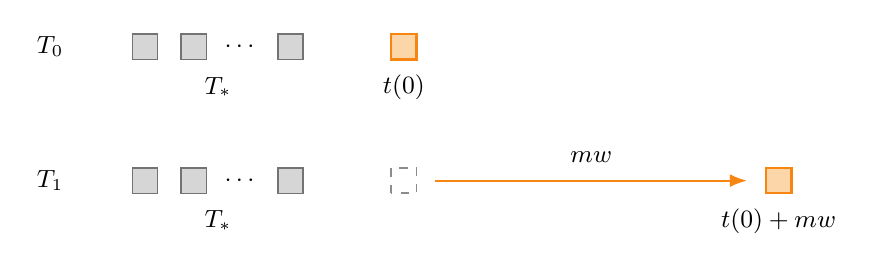
\begin{tikzpicture}[
  x=1cm,y=1cm,
  every node/.style={font=\small},
  common/.style={draw=black!55,fill=black!16,line width=.5pt},
  marked/.style={draw=BurntOrange,fill=BurntOrange!30,line width=.9pt}
]
  \node[anchor=east] at (0.8,1.35) {$T_0$};
  \node[anchor=east] at (0.8,-0.35) {$T_1$};

  \foreach \y in {1.35,-0.35} {
    \draw[common] (1.55,\y-.16) rectangle (1.87,\y+.16);
    \draw[common] (2.17,\y-.16) rectangle (2.49,\y+.16);
    \node at (2.94,\y) {$\cdots$};
    \draw[common] (3.40,\y-.16) rectangle (3.72,\y+.16);
    \node at (2.64,\y-.51) {$T_*$};
  }

  \draw[marked] (4.84,1.19) rectangle (5.16,1.51);
  \node at (5,0.84) {$t(0)$};

  \draw[draw=black!45,dashed,line width=.6pt]
    (4.84,-.51) rectangle (5.16,-.19);
  \draw[-{Latex[length=2.2mm]},line width=.8pt,BurntOrange]
    (5.40,-.35) -- node[above=3pt,text=black] {$mw$} (9.36,-.35);
  \draw[marked] (9.60,-.51) rectangle (9.92,-.19);
  \node at (9.76,-.86) {$t(0)+mw$};
\end{tikzpicture}
\caption{Schematic of the marked-point switch, without depicting the
actual positions or scale.  The gray marks represent the same common
set $T_*$ in both rows.  The marked point moves from $t(0)$ to
$t(0)+mw$; the dashed outline shows its former location.  The marks
may also denote unit-cube thickenings.  In a grid assembly this switch
gives the kernel-invariance identity \eqref{geom:kernel-invariance}.}
\label{geom:fig-switch}
\end{figure}


Our final discrete tile is
\begin{equation}
 T=T_1\cup\bigcup_{u\in U\setminus\{0\}}(mu+T_0),
 \qquad \Omega=T+[0,1]^3.
 \label{geom:large-tile}
\end{equation}
The finite union defining $T$ is disjoint.  To see this, equality of
two points first forces equality of their residue labels $v$ modulo
$m$.  For $v\ne0$, the points are $mu+t(v)$, and equality forces
the same $u$.  For $v=0$, the unmarked points are
$mu+t(0)$ with $u\in U\setminus\{0\}$, while the marked point is
$mw+t(0)$.  They are all distinct by
\cref{geom:representatives-U}.  In particular, $|T|=|U|m^3$.

Write
\[
 \Omega_i=T_i+[0,1]^3\quad(i=0,1),\qquad
 \Omega_*=T_*+[0,1]^3.
\]
Each $\Omega_i$ has volume $m^3$, and their common subset $\Omega_*$
has positive volume $m^3-1$.  Unit cubes with distinct integer lower
corners have disjoint interiors, so the decomposition of $T$ in
\cref{geom:large-tile} gives the corresponding decomposition of
$\Omega$ up to null boundaries.
We call the translation vector $c$ the center of the copy $c+T_i$
or $c+\Omega_i$.

\subsection{Existence of a tiling}

\begin{proposition}
\label{geom:existence}
The tile $T$ tiles $\Z^3$, and $\Omega$ tiles $\R^3$ up to null sets.
\end{proposition}

\begin{proof}
Let $A\oplus F=\Gamma$ be a tiling from \cref{stack:cyclic}, and put
$B=\pi^{-1}(A)$.  Then $B+w=B$.  Also
$B\oplus U=\Z^3$: for any $g\in\Z^3$, the unique representation of
$\pi(g)$ in $A+F$ determines a unique $u\in U$, and then $g-u\in B$
is the unique possible other summand.

Place copies of $T$ at all translations in $mB$.  Their constituent
copies of $T_0$ or $T_1$ have centers $m(b+u)$, for $b\in B$ and
$u\in U$.  Since $B\oplus U=\Z^3$, there is exactly one such center
at every point of $m\Z^3$.  Its type is $1$ precisely at the centers
$mB$, because the type-$1$ piece corresponds to $u=0$.

The assembly with $T_0$ at every center in $m\Z^3$ tiles $\Z^3$
exactly: each integer vector has a unique residue label $v$ and a
unique expression $ma+t(v)$.  Switching to type $1$ at the centers
$mB$ removes the marked points
\[
 t(0)+mB
\]
and inserts
\[
 t(0)+m(B+w)=t(0)+mB.
\]
The insertion is a bijective relocation, so all multiplicities
remain one.  This proves $mB\oplus T=\Z^3$.  Thickening by unit
cubes gives an almost-everywhere tiling by $\Omega$ with the same
translation set: away from the integer coordinate planes, every
point belongs to the interior of one integer unit cube.
\end{proof}

\subsection{Rigidity for real translation vectors}

We next show why arbitrary real translations cannot produce a
periodic tiling.  The marked-point modification has two roles.
The common part forces the centers of the small pieces onto one
grid, and the moved point then forces invariance under the kernel
direction $w$.

\begin{lemma}[Rounding in the closed box]
\label{geom:rounding}
Let $m\geq2$, and suppose that $\delta\in\R^3$ satisfies
$\norm{\delta}_\infty\leq m$ and $\delta\notin m\Z^3$.  There is
$d\in\Z^3\setminus m\Z^3$ such that
\[
 \norm{d}_\infty\leq m,
 \qquad \norm{\delta-d}_\infty<1.
\]
\end{lemma}

\begin{proof}
If $\delta$ is integral, use $d=\delta$.  Otherwise, keep every
integer coordinate unchanged and round each noninteger coordinate
either down or up.  Both choices lie in $[-m,m]$, since the
endpoints are integers, and both are at distance strictly less than
one from the original coordinate.  In at least one noninteger
coordinate choose a rounding which is not a multiple of $m$.
Such a choice exists because two consecutive integers cannot both
be multiples of $m\geq2$.  The resulting $d$ is not in $m\Z^3$.
Coordinates of $\delta$ equal to $m$ or $-m$ are left unchanged, so
the strict distance estimate also holds on the boundary of the box.
\end{proof}

\begin{lemma}[A periodic assembly has grid centers]
\label{geom:grid}
Suppose copies $c+\Omega_{\iota(c)}$, with types
$\iota(c)\in\{0,1\}$, form an almost-everywhere tiling of $\R^3$.
Assume the assembly, including its types, is invariant under a
full-rank lattice $\Lambda\subset\R^3$.  Then the set $C$ of centers
is $c_0+m\Z^3$ for some $c_0\in\R^3$.
\end{lemma}

\begin{proof}
First, two constituent copies cannot have the same center, because
both contain the positive-volume common part $\Omega_*$.  Thus the
centers and their types are unambiguous.  We claim that distinct
centers $c,c'$ satisfy
\begin{equation}
 \norm{c'-c}_\infty\leq m
 \quad\Longrightarrow\quad c'-c\in m\Z^3.
 \label{geom:nearby-centers}
\end{equation}
If $\delta=c'-c$ violated this assertion, \cref{geom:rounding} would
give a vector $d$ in the difference set in
\eqref{geom:difference-property} with
$\norm{\delta-d}_\infty<1$.  Write $d=t-t'$ for $t,t'\in T_*$.  The
two common-part unit cubes
\[
 c+t+[0,1]^3,\qquad c'+t'+[0,1]^3
\]
have lower corners whose coordinate differences have absolute
value strictly less than one.  Their intersection therefore has
positive volume, contradicting the tiling property.  This proves
\cref{geom:nearby-centers}.

In particular, distinct centers have sup-norm distance at least
$m$: a nonzero vector in $m\Z^3$ cannot have smaller sup norm.
The set $C$ is consequently uniformly separated and locally finite.
The auxiliary closed cubes
\[
 Q_c=c+[-m/2,m/2]^3\qquad(c\in C)
\]
have disjoint interiors.  Each has volume $m^3$, equal to the
volume of either constituent type.

We use periodicity to show that these auxiliary cubes cover.  Let
$P$ be a bounded half-open fundamental parallelepiped for $\Lambda$.
There are finitely many centers modulo $\Lambda$, by local
finiteness; choose representatives $c_1,\ldots,c_r$.  Their types
$\iota_1,\ldots,\iota_r$ are preserved under $\Lambda$.  Integrating
the constituent tiling over $P$ gives
\begin{align*}
 |P|
 &=\int_P\sum_{j=1}^r\sum_{\lambda\in\Lambda}
       \mathbf{1}_{c_j+\lambda+\Omega_{\iota_j}}(x)\,dx\\
 &=\sum_{j=1}^r|\Omega_{\iota_j}|=rm^3.
\end{align*}
For the second equality, translate the integration domains by
$-\lambda$ and use that $\{P-\lambda:\lambda\in\Lambda\}$ partitions
$\R^3$ up to boundaries.  Nonnegative summands justify the exchange
of summation and integration.

The same calculation for the auxiliary cubes gives
\[
 \int_P\sum_{c\in C}\mathbf{1}_{Q_c}(x)\,dx=rm^3=|P|.
\]
The integrand is at most one almost everywhere, because the cubes
have disjoint interiors; their countably many boundaries are null.
It is therefore one almost everywhere on $P$, and periodicity gives
almost-everywhere coverage of $\R^3$.  The family of closed cubes
$\{Q_c\}_{c\in C}$ is locally finite, so its union is closed.  A
point outside the union would have an open neighborhood of positive
volume outside it, contradicting almost-everywhere coverage.  Thus
the cubes cover every point of $\R^3$.

Their intersection graph is connected.  Indeed, if one graph
component were separated from the remaining components, the unions
of their respective cubes would be disjoint nonempty closed sets
covering $\R^3$.  Both unions are closed because they are subfamilies
of a locally finite family of closed sets.  They would disconnect
$\R^3$, which is impossible.  Whenever $Q_c$ and $Q_{c'}$ intersect,
$\norm{c'-c}_\infty\leq m$, so \cref{geom:nearby-centers} puts their
difference in $m\Z^3$.  Following paths in the intersection graph
therefore puts every center in one coset $c_0+m\Z^3$.

No point of that coset can be missing.  The interior of the
side-$m$ cube at a missing grid point is disjoint from all side-$m$
cubes at the other grid points and would be uncovered.  Hence
$C=c_0+m\Z^3$.
\end{proof}

\subsection{Kernel invariance and descent}

\begin{proposition}
\label{geom:no-periodic}
The Euclidean tile $\Omega$ has no almost-everywhere translational
tiling whose translation set is invariant under a full-rank lattice
in $\R^3$.
\end{proposition}

\begin{proof}
Suppose, to the contrary, that $\mathcal A\subset\R^3$ is such a
translation set and that $\mathcal A+\Lambda=\mathcal A$ for a
full-rank lattice $\Lambda$.  Distinct vectors of $\mathcal A$ have
sup-norm distance at least one: otherwise their translates of a fixed
unit cube in $\Omega$ would overlap in positive volume.  Hence
$\mathcal A$ is countable.  Decompose every translated copy of
$\Omega$ using \cref{geom:large-tile}.  A copy at $a\in\mathcal A$
has a type-$1$ constituent centered at $a$ and type-$0$ constituents
centered at $a+mu$ for $u\in U\setminus\{0\}$.  The constituents
form an almost-everywhere tiling and inherit the lattice periods,
including their types.  No two constituents have the same center,
as observed in the proof of \cref{geom:grid}.  Consequently the map
\begin{equation}
 \mathcal A\times U\longrightarrow C,\qquad(a,u)\longmapsto a+mu
 \label{geom:center-decomposition}
\end{equation}
is a bijection, and the type-$1$ centers are exactly $\mathcal A$.

By \cref{geom:grid}, $C=c_0+m\Z^3$.  Translate the entire assembly
by $-c_0$, which does not change its period lattice, and henceforth
write $C=m\Z^3$.  There is a set $B'\subset\Z^3$ such that
$\mathcal A=mB'$.  Let $b(a)=\mathbf{1}_{B'}(a)$; this records the
type at the center $ma$.  The bijection
\eqref{geom:center-decomposition}, divided by $m$, gives
\begin{equation}
 B'\oplus U=\Z^3.
 \label{geom:upstairs-tiling}
\end{equation}

Consider the open unit cell with lower corner $t(0)+ma$, for any
$a\in\Z^3$.  Since all constituent centers and all voxel positions
are integral, a unit cube can meet the interior of this cell only
if it has the same lower corner.  The residues modulo $m$ then
exclude every common-part point $t(v)$ with $v\ne0$.  There are
exactly two possible sources: the unshifted marked point from
type $0$ at $ma$, or the moved marked point from type $1$ at
$m(a-w)$.  The coverage multiplicity on this open cell is therefore
\[
 1-b(a)+b(a-w).
\]
The almost-everywhere tiling makes it one.  Thus $b(a)=b(a-w)$ for
every $a$, or equivalently
\begin{equation}
 B'+w=B'.
 \label{geom:kernel-invariance}
\end{equation}
This also gives invariance under every element of $\ker\pi=\Z w$.

The set $B'$ is fully periodic in the discrete sense.  It is
nonempty, and $\mathcal A=mB'\subset m\Z^3$.  For $a_0\in\mathcal A$
and any $\lambda\in\Lambda$, both $a_0$ and $a_0+\lambda$ belong to
$m\Z^3$, so $\lambda\in m\Z^3$.  Hence
$L=m^{-1}\Lambda$ is a rank-three lattice contained in $\Z^3$ and
preserves $B'$.  Such an integer lattice has finite index: the
matrix formed by an integer basis has nonzero integer determinant,
whose absolute value is its index.  In particular, $L\leq\Z^3$ is
a finite-index period subgroup of $B'$.

We finally descend the exact tiling
\eqref{geom:upstairs-tiling} to the quotient.  Fix $\gamma\in\Gamma$
and any lift $g\in\Z^3$.  For each $u\in U$, there is a
representation
\[
 \gamma=\alpha+\pi(u),\qquad \alpha\in\pi(B'),
\]
if and only if $g-u\in B'$.  One direction follows by applying
$\pi$.  For the other, if $\alpha=\pi(b_0)$ with $b_0\in B'$, then
$g-u-b_0\in\ker\pi$; \cref{geom:kernel-invariance} therefore puts
$g-u$ in $B'$.  By \cref{geom:upstairs-tiling}, exactly one $u$ has
this property, and $\pi$ is injective on $U$.  Thus
\[
 \pi(B')\oplus\pi(U)=\Gamma.
\]
This quotient tiling is fully periodic.  Indeed, $\pi(L)$ preserves
$\pi(B')$, and the surjection
$\Z^3/L\to\Gamma/\pi(L)$ shows that $\pi(L)$ has finite index.
Since $\pi(U)=F$, this contradicts \cref{stack:cyclic}.
\end{proof}

\begin{proof}[Completion of the proof of \cref{thm:main}]
The finite nonempty tile $T$ from \cref{geom:large-tile} and its
closed unit-cube thickening $\Omega$ admit the tilings in
\cref{geom:existence}.  The Euclidean tiling cannot be fully
periodic by \cref{geom:no-periodic}.  If a discrete tiling of $T$
had a finite-index period subgroup in $\Z^3$, thickening its unit
cells would give an almost-everywhere tiling of $\Omega$ invariant
under the same subgroup, viewed as a full-rank lattice in $\R^3$.
This is also excluded by \cref{geom:no-periodic}, proving both
claims.
\end{proof}

\begin{remark}[Finite selection of the tile data]
The finite data in the construction can be selected by terminating
finite searches. The primes can be selected successively by trial division. The tiling
tests involve maps between finite sets. Lemmas~\ref{stack:partition}
and~\ref{geom:random-representatives} give explicit inequalities
under which a suitable finite coloring or residue transversal exists;
exhaustive search then selects one. This describes
the finite tile itself. The infinite tiling that proves existence is
instead specified by the last-nonzero-digit function. No practical bound
on the size of the finite construction is required.
\end{remark}


\renewcommand{\bibfont}{\small}
\bibliographystyle{plainnat}
\bibliography{references}
\end{document}
